% Options for packages loaded elsewhere
\PassOptionsToPackage{unicode}{hyperref}
\PassOptionsToPackage{hyphens}{url}
%
\documentclass[
]{book}
\usepackage{amsmath,amssymb}
\usepackage{lmodern}
\usepackage{iftex}
\ifPDFTeX
  \usepackage[T1]{fontenc}
  \usepackage[utf8]{inputenc}
  \usepackage{textcomp} % provide euro and other symbols
\else % if luatex or xetex
  \usepackage{unicode-math}
  \defaultfontfeatures{Scale=MatchLowercase}
  \defaultfontfeatures[\rmfamily]{Ligatures=TeX,Scale=1}
\fi
% Use upquote if available, for straight quotes in verbatim environments
\IfFileExists{upquote.sty}{\usepackage{upquote}}{}
\IfFileExists{microtype.sty}{% use microtype if available
  \usepackage[]{microtype}
  \UseMicrotypeSet[protrusion]{basicmath} % disable protrusion for tt fonts
}{}
\makeatletter
\@ifundefined{KOMAClassName}{% if non-KOMA class
  \IfFileExists{parskip.sty}{%
    \usepackage{parskip}
  }{% else
    \setlength{\parindent}{0pt}
    \setlength{\parskip}{6pt plus 2pt minus 1pt}}
}{% if KOMA class
  \KOMAoptions{parskip=half}}
\makeatother
\usepackage{xcolor}
\IfFileExists{xurl.sty}{\usepackage{xurl}}{} % add URL line breaks if available
\IfFileExists{bookmark.sty}{\usepackage{bookmark}}{\usepackage{hyperref}}
\hypersetup{
  pdftitle={Microéconomie 2},
  pdfauthor={Elias Bouacida; Antoine Terracol},
  hidelinks,
  pdfcreator={LaTeX via pandoc}}
\urlstyle{same} % disable monospaced font for URLs
\usepackage{longtable,booktabs,array}
\usepackage{calc} % for calculating minipage widths
% Correct order of tables after \paragraph or \subparagraph
\usepackage{etoolbox}
\makeatletter
\patchcmd\longtable{\par}{\if@noskipsec\mbox{}\fi\par}{}{}
\makeatother
% Allow footnotes in longtable head/foot
\IfFileExists{footnotehyper.sty}{\usepackage{footnotehyper}}{\usepackage{footnote}}
\makesavenoteenv{longtable}
\usepackage{graphicx}
\makeatletter
\def\maxwidth{\ifdim\Gin@nat@width>\linewidth\linewidth\else\Gin@nat@width\fi}
\def\maxheight{\ifdim\Gin@nat@height>\textheight\textheight\else\Gin@nat@height\fi}
\makeatother
% Scale images if necessary, so that they will not overflow the page
% margins by default, and it is still possible to overwrite the defaults
% using explicit options in \includegraphics[width, height, ...]{}
\setkeys{Gin}{width=\maxwidth,height=\maxheight,keepaspectratio}
% Set default figure placement to htbp
\makeatletter
\def\fps@figure{htbp}
\makeatother
\setlength{\emergencystretch}{3em} % prevent overfull lines
\providecommand{\tightlist}{%
  \setlength{\itemsep}{0pt}\setlength{\parskip}{0pt}}
\setcounter{secnumdepth}{5}
\usepackage{booktabs}
\usepackage[french]{babel}
\ifLuaTeX
  \usepackage{selnolig}  % disable illegal ligatures
\fi
\usepackage[]{natbib}
\bibliographystyle{plainnat}

\title{Microéconomie 2}
\author{Elias Bouacida \and Antoine Terracol}
\date{2021-09-20}

\usepackage{amsthm}
\newtheorem{theorem}{Théorème}[chapter]
\newtheorem{lemma}{Lemme}[chapter]
\newtheorem{corollary}{Corollaire}[chapter]
\newtheorem{proposition}{Proposition}[chapter]
\newtheorem{conjecture}{Conjecture}[chapter]
\theoremstyle{definition}
\newtheorem{definition}{Définition}[chapter]
\theoremstyle{definition}
\newtheorem{example}{Exemple}[chapter]
\theoremstyle{definition}
\newtheorem{exercise}{Exercice}[chapter]
\theoremstyle{definition}
\newtheorem{hypothesis}{Hypothèse}[chapter]
\theoremstyle{remark}
\newtheorem*{remark}{Remarque}
\newtheorem*{solution}{Solution}
\begin{document}
\maketitle

{
\setcounter{tocdepth}{1}
\tableofcontents
}
\hypertarget{microuxe9conomie-2}{%
\chapter{Microéconomie 2}\label{microuxe9conomie-2}}

Cours de microéconomie 2 en licence 2 à l'université Paris 8, donné par Antoine Terracol et Elias Bouacida.\\
Ce dépôt contient les notes de cours ainsi que les corrigés des exercices.

\hypertarget{thuxe8mes}{%
\section{Thèmes}\label{thuxe8mes}}

Les principaux thèmes abordés dans ce cours sont les suivants :

\begin{itemize}
\tightlist
\item
  structures de marché
\item
  pouvoir de marché
\item
  principes de tarification
\item
  comportements stratégiques
\item
  problèmes d'information
\end{itemize}

L'idée générale est de dépasser le cadre de la concurrence pure et parfaite et de se rapprocher un peu du \emph{monde réel} en levant certaines hypothèses de la concurrence pure et parfaite.

\hypertarget{bibliographie}{%
\section{Bibliographie}\label{bibliographie}}

Le cours ne nécessite pas de se référer à un manuel.
Néanmoins, pour ceux qui souhaitent des éclairages différents sur les notions abordés, voici quelques références utiles:

\begin{itemize}
\tightlist
\item
  \citet{varian2015} \emph{Introduction à la microéconomie}
\item
  \citet{varian2008} \emph{Analyse Microéconomique}
\item
  \citet{pindyck2012} \emph{Microéconomie}
\item
  \citet{jeleva2014} \emph{Microéconomie}
\end{itemize}

Et enfin une référence avancée, pour ceux qui cherchent les fondements mathématiques (en anglais):

\begin{itemize}
\tightlist
\item
  \citet{mas1995} \emph{Microeconomic Theory}
\end{itemize}

\hypertarget{plan-du-cours}{%
\section{Plan du cours}\label{plan-du-cours}}

\begin{enumerate}
\def\labelenumi{\arabic{enumi}.}
\tightlist
\item
  Rappels sur la concurrence pure et parfaite
\item
  Monopoles

  \begin{itemize}
  \tightlist
  \item
    Monopoles simples
  \item
    Monopoles discriminants
  \item
    Pouvoir de marché et principes de tarification
  \end{itemize}
\item
  Oligopoles

  \begin{itemize}
  \tightlist
  \item
    Duopoles à la Cournot
  \item
    Duopoles à la Stackelberg
  \item
    Collusion
  \end{itemize}
\end{enumerate}

\hypertarget{rappels-le-marchuxe9-en-concurrence-pure-et-parfaite}{%
\chapter{Rappels : le marché en concurrence pure et parfaite}\label{rappels-le-marchuxe9-en-concurrence-pure-et-parfaite}}

\hypertarget{les-hypothuxe8ses-de-la-concurrence-pure-et-parfaite-cpp}{%
\section{Les hypothèses de la concurrence pure et parfaite (CPP)}\label{les-hypothuxe8ses-de-la-concurrence-pure-et-parfaite-cpp}}

Il y a 5 hypothèses qui définissent la concurrence pure et parfaite :

\begin{enumerate}
\def\labelenumi{\arabic{enumi}.}
\tightlist
\item
  Atomicité des agents
\item
  Information parfaite
\item
  Mobilité parfaite des facteurs de production
\item
  Homogénéité des biens
\item
  Libre entrées et sorties des marchés
\end{enumerate}

L'hypothèse 1 implique que personne n'a d'influence \emph{individuellement} sur les prix.
En d'autres termes, chaque acteur est petit face au marché et considère le prix du marché comme une \emph{donnée} qu'il ne peut pas influencer.
On dit que les agents sont \emph{price-taker} sur le marché.

L'hypothèse 2 signifie que tous les acteurs disposent de toutes les informations pertinentes pour prendre leurs décisions.
Il n'y a, par exemple, pas de coût de recherche d'information.

L'hypothèse 3 garantit l'homogénéité spatiale du prix des facteurs.
Les différences de coûts entre producteurs ne peuvent donc être dus qu'au différence technologique entre ceux-ci, et non à une différence de coût des facteurs de production.

L'hypothèse 4 qu'il n'y notamment pas d'effet des marques.

L'hypothèse 5 qu'il n'y pas de barrière à l'entrée dans le marché.
Concrètement, cela implique qu'il est impossible de faire du bénéfice sur la dernière unité vendue en concurrence pure et parfaite, sinon un concurrent pourrait entrer sur le marché et faire des bénéfices.

La violation d'une de ces hypothèses nous fait sortir du cadre de la CPP et confère un \emph{pouvoir de marché} aux entreprises en place.

\hypertarget{luxe9quilibre-de-marchuxe9}{%
\section{L'équilibre de marché}\label{luxe9quilibre-de-marchuxe9}}

\emph{Demande agrégée (D)} : Somme des demandes individuelles pour chaque niveau de prix.

\emph{Offre agrégée (S)} : Somme des offres individuelles pour chaque niveau de prix.

L'équilibre de marché se fait à l'intersection entre S et D (quand S=D).

\begin{figure}
\centering
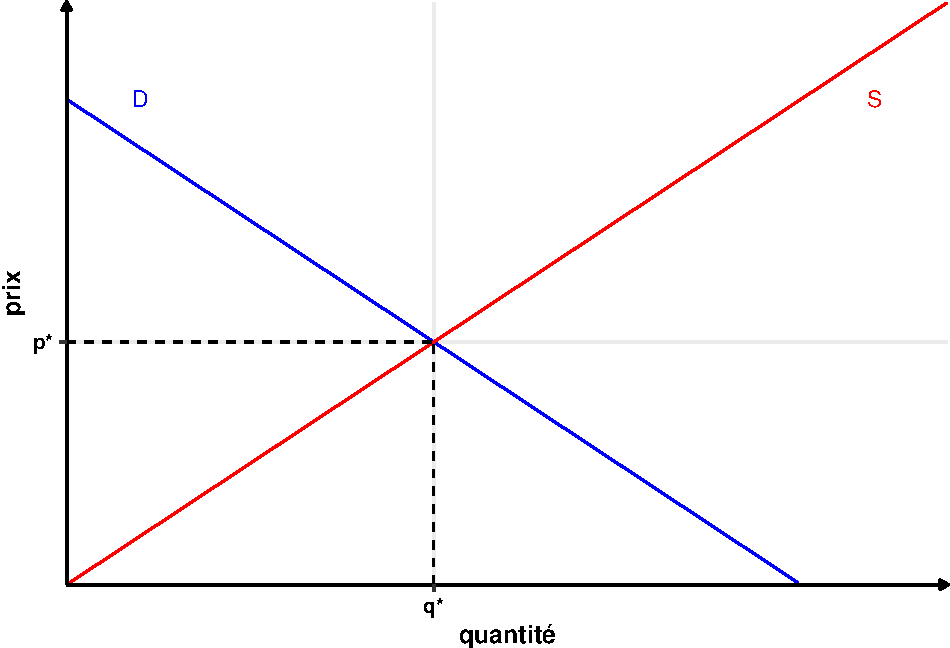
\includegraphics{_main_files/figure-latex/marche-1.pdf}
\caption{\label{fig:marche}Equilibre de marché.}
\end{figure}

La courbe de demande correspond à la suite des prix de réserve des individus, c'est-à-dire aux prix maximal que chaque individu est prêt à payer pour obtenir une unité \emph{supplémentaire} du bien.

La courbe d'offre correspond à la série des coûts marginaux de production, c'est-à-dire les prix minimaux auxquels les producteurs souhaitent vendre une unité supplémentaire du bien.

La vente de toutes les unités jusqu'à la quantité d'équilibre \(q^*\) au prix \(p^*\) procure un \emph{surplus} aux agents économiques.

\begin{figure}
\centering
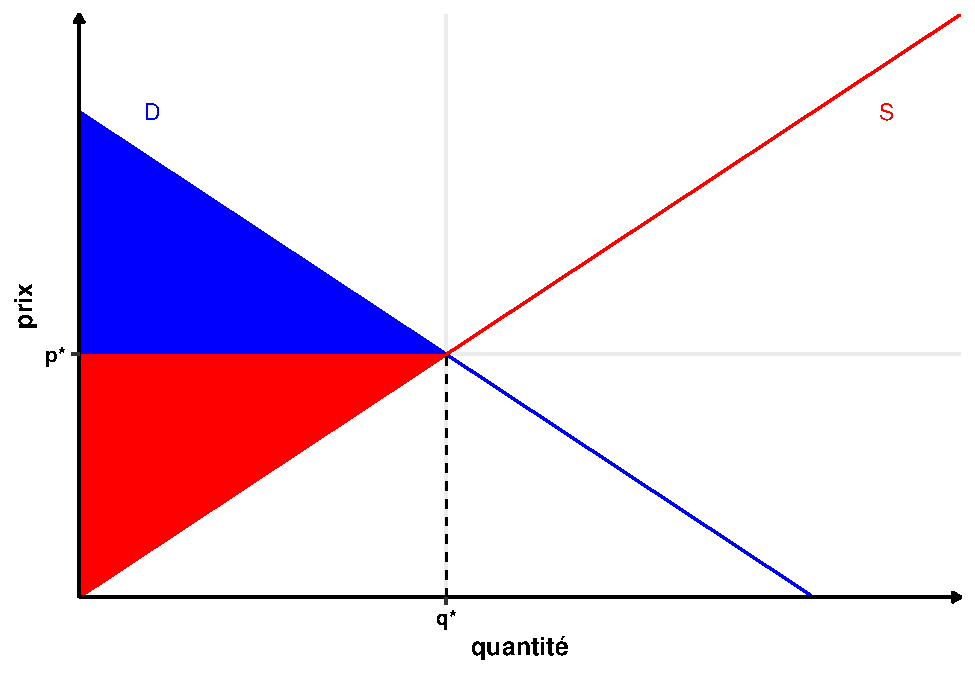
\includegraphics{_main_files/figure-latex/surplus-1.pdf}
\caption{\label{fig:surplus}Surplus des consommateurs et des producteurs.}
\end{figure}

\textbf{Propriétés :}

\begin{itemize}
\tightlist
\item
  L'équilibre en CPP est celui qui \textbf{maximise} le \emph{surplus total}.
  Tout autre couple prix/quantité abouti à un surplus total plus faible.
\item
  L'équilibre de CPP est \emph{Pareto-optimal}, i.e., il est impossible d'améliorer la situation d'un agent sans détériorer celle d'un autre.
  C'est ce qu'on appelle le \emph{premier théorème du bien-être}.
\end{itemize}

Ces propriétés font de la CPP une ``référence'' par rapport à laquelle on peut comparer les résultats des autres structures de marché.

\hypertarget{perception-par-les-agents-isoluxe9s}{%
\section{Perception par les agents isolés}\label{perception-par-les-agents-isoluxe9s}}

L'hypothèse d'atomicité indique que les agents individuels sont isolés au sein d'un très grand nombre d'autres agents.
Ainsi, aucun agent n'a d'influence sur le prix s'il modifie son comportement.
Une conséquence directe est que le comportement des autres agents est perçu comme étant infiniment élastique.
C'est-à-dire qu'un producteur sait qu'au prix de marché, il pourra vendre toute sa production, mais que s'il pratique un prix même légèrement plus élevé, il ne vendra \textbf{rien}.
Il perçoit ainsi une demande infiniment élastique au prix, au niveau du prix \(p^*\).

\begin{figure}

{\centering 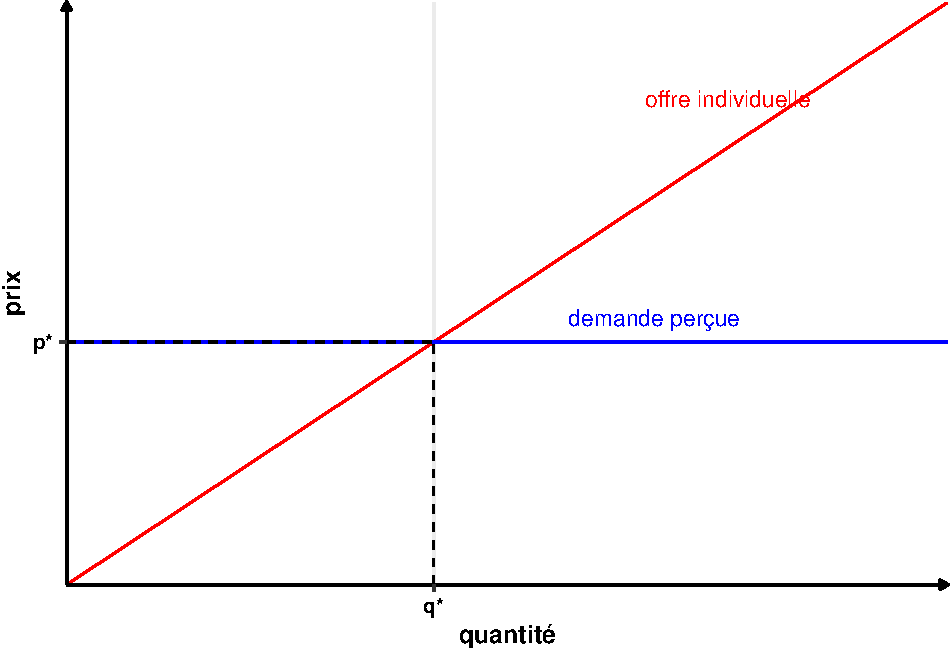
\includegraphics{_main_files/figure-latex/elasticite-1} 

}

\caption{Perception de la demande globale par un producteur isolé.}\label{fig:elasticite}
\end{figure}

Dans ce graphique, \(q^*\) représente la production optimale de ce producteur quand il est seul.

\hypertarget{le-monopole}{%
\chapter{Le monopole}\label{le-monopole}}

\begin{definition}[Monopole]
Un \emph{monopole} est sur un marché donné l'unique entreprise qui produit le bien.
\end{definition}

C'est le cas extrême opposé à la concurrence pure et parfaite, du côté du producteur.
Il est intéressant à étudier car il nous renseigne sur les principaux aspects du comportement des entreprises dans les cas intermédiaires.

Il y a de nombreuses raisons qui aboutissent à l'existence de monopoles.
Les principales sont:

\begin{itemize}
\tightlist
\item
  Légales, à cause de réglementation particulières.
  C'est ce qu'on appelle en général des professions réglementées, comme les avocats, les bureaux de tabac, les taxis\ldots{}
\item
  Légales, à cause des brevets sur une technologie données (industrie pharmaceutique\ldots)
\item
  Historique, le premier arrivé
\item
  Monopoles \emph{naturels}: en présence d'économies d'échelles, produire une quantité donnée revient moins cher avec une seule firme qu'avec plusieurs.
  C'est notamment les cas des industries où il faut installer des réseaux (chemins de fer, électricité, téléphone, etc).
  Plus généralement, les industries avec des coûts fixes / coûts d'entrées très élevées aboutissent à des formes proches du monopole naturel (sidérurgie, automobile\ldots)
\item
  Exclusivité sur la production de certaines matières premières (cuivre au Chili, terres rares en Chine,\ldots)
\item
  Coalitions créant un cartel
\end{itemize}

\hypertarget{recette-et-recette-marginale}{%
\section{Recette et recette marginale}\label{recette-et-recette-marginale}}

\hypertarget{duxe9finition}{%
\subsection{Définition}\label{duxe9finition}}

A la différence du cas de la concurrence pure et parfaite, le monopole perçoit la courbe de demande agrégée, et non plus celle avec une élasticité infinie.
Le choix de la quantité qu'il met sur le marché modifie le prix auquel il pourra vendre sa production, et il le sait.\\
Il va choisir \textbf{un} des paramètres du couple \((q, P(q))\), et l'autre en découlera, à travers la demande \(P(q)\).
Autrement dit, s'il choisit \(q\), \(P(q)\) sera déterminé par la demande (inverse).
Si, au contraire, il choisit \(P\), \(q\) sera déterminé par la demande.

En CPP, la recette totale du producteur individuel était \(R(q) = q\cdot P(q^*)\), où \(x\) est sa production individuel, \(q^*\) la quantité d'équilibre sur le marché (résultat de la production de \emph{toutes} les entreprises présentes sur le marché) et \(P(q^*)=p^*\) est le prix d'équilibre.

En monopole, le prix dépend de la production du monopole (ou l'inverse, peu importe) :
\[
R(q) = q\cdot P(q)
\]

\begin{definition}[Recette marginale]
La recette marginale correspond à la variation de la recette totale provoquée par une ``petite'' variation \(\Delta q\) de la quantité mise sur le marché.

\[R_m(q) = \lim_{\Delta q\to 0} \frac{R(q+\Delta q)-q}{\Delta q} = \frac{d R(q)}{d q} = R'(q)\]
\end{definition}

La recette marginale est mesurée en unité monétaire par unité de bien (comme le prix).

\hypertarget{recette-marginale-et-courbe-de-demande}{%
\subsection{Recette marginale et courbe de demande}\label{recette-marginale-et-courbe-de-demande}}

Comme la courbe de demande est décroissante (l'élasticité prix de la demande est négative \(\varepsilon_{q/p} <0\)), \(P(q)\) et \(q\) ont une relation inverse.
Autrement dit, si \(q\) augmente, alors \(p\) baisse, et réciproquement.

Cela implique que la recette totale va augmenter ou baisser suivant les propriétés de la courbe de demande.

\begin{figure}
\centering
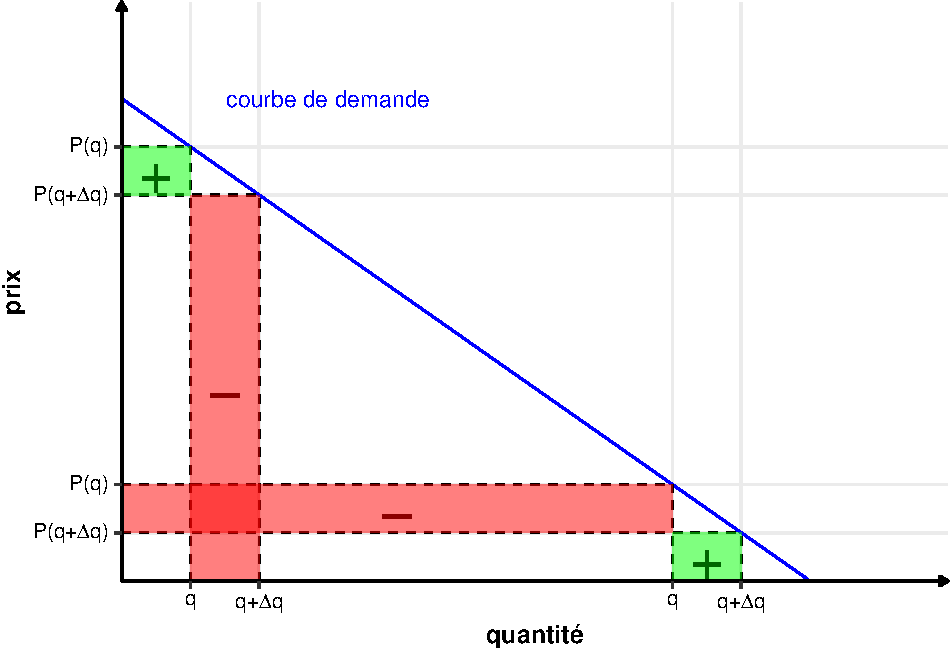
\includegraphics{_main_files/figure-latex/recette_marginale-1.pdf}
\caption{(\#fig:recette\_marginale)Recette marginale d'un monopole.}
\end{figure}

Quel est le paramètre important de la courbe de demande qui détermine si le revenu \(R\) augmente ou diminue (càd si \(R_m\) est positive ou négative) ?

\begin{align*}
R(q) & = qP(q)\\
R_m(q)& = \frac{dR(q)}{dq} \\
& = \frac{d (qP(q))}{dq} \\
& = P(q) + q\frac{d P(q)}{dq} \\
& = P(q)\left(1 + \frac{q}{P(q)}\frac{d P(q)}{dq} \right)\\
& = P(q)\left(1 + \frac{1}{\varepsilon_{q/p}}\right)
\end{align*}

\emph{Rappel :} \(\frac{P(q)}{q}\frac{dq}{dP(q)} = \varepsilon_{q/p} <0\)

\begin{equation}
R_m(q) = P(q)\left(1 - \frac{1}{|\varepsilon_{q/p}|}\right)\\
\label{eq:rm}
\end{equation}

De l'équation \eqref{eq:rm}, on voit clairement que le signe de \(R_m\) dépend de l'élasticité prix de la demande.

\begin{enumerate}
\def\labelenumi{\arabic{enumi}.}
\tightlist
\item
  Si la demande est élastique (\(|\varepsilon_{q/p}|>1\)), alors \(R_m(q)>0\), donc si la quantité augmente, le revenu augmente.
\item
  Si la demande est inélastique (\(|\varepsilon_{q/p}|<1\)), alors \(R_m(q)<0\), donc si la quantité augmente, le revenu diminue.
\end{enumerate}

\begin{figure}
\centering
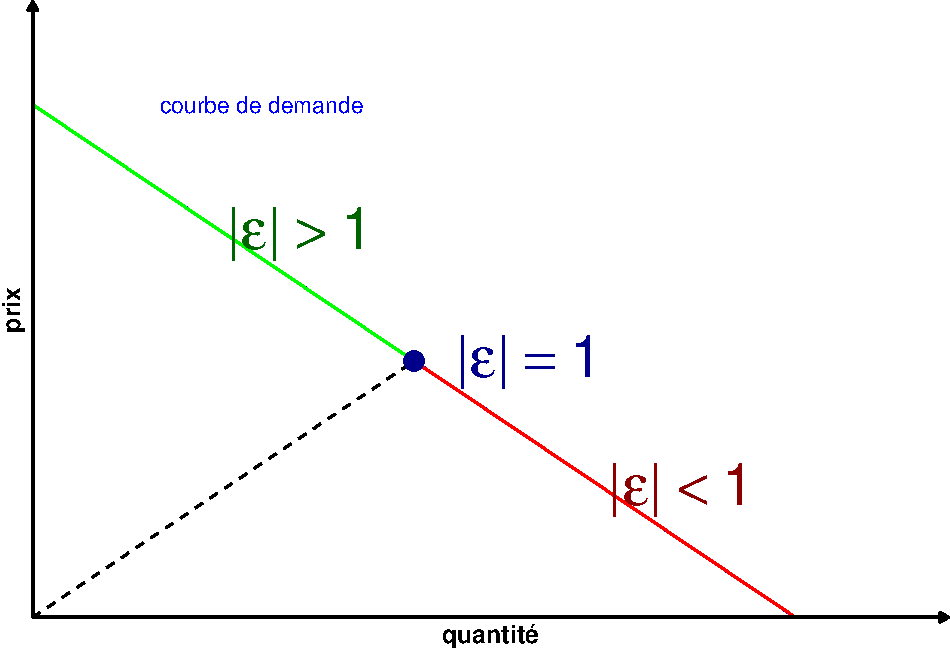
\includegraphics{_main_files/figure-latex/monopoleelasticite-1.pdf}
\caption{\label{fig:monopoleelasticite}Elasticité et profit.}
\end{figure}

\hypertarget{repruxe9sentation-graphique}{%
\subsection{Représentation graphique}\label{repruxe9sentation-graphique}}

La courbe de recette marginale est toujours située en-dessous de la courbe de demande :
\[
R_m(q) = P(q) + q\frac{d P(q)}{dq} < P(q)
\]
et \(\frac{d P(q)}{dq}\) est négative (la demande est décroissante quand le prix augmente).

\hypertarget{exemple-avec-une-courbe-de-demande-linuxe9aire}{%
\subsubsection{Exemple avec une courbe de demande linéaire}\label{exemple-avec-une-courbe-de-demande-linuxe9aire}}

Prenons maintenant l'exemple d'une courbe de demande linéaire quelconque \(P(q) = a-bq\) (\(a\) et \(b\) sont des paramètres quelconques).
On obtient alors \(R_m(q) = a-2bq\) (et \(R(q) = aq-bq^2\)).\\
Dans le cas linéaire, le revenu marginal est une droite de pente deux fois plus forte que la demande, et ayant la même ordonnée à l'origine.
La recette marginale divise en deux tout segment horizontal entre l'axe des ordonnées et la courbe de demande.

\begin{figure}
\centering
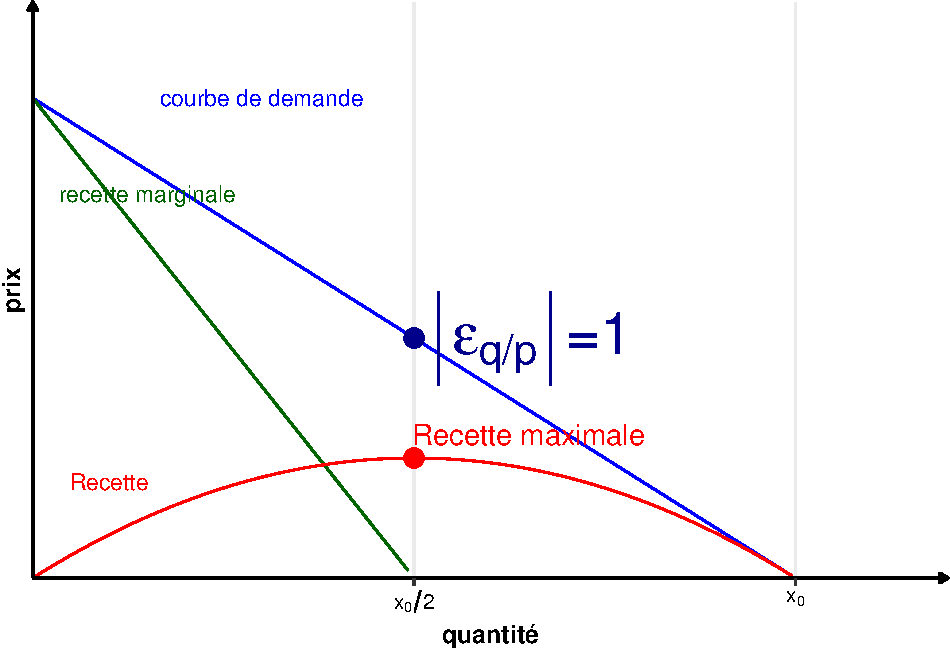
\includegraphics{_main_files/figure-latex/recettemarginale-1.pdf}
\caption{\label{fig:recettemarginale}Elasticité et recette.}
\end{figure}

La recette maximale est atteinte lorsque la valeur absolue de l'élasticité prix de la demande est égale à 1 (\(|\varepsilon_{q/p}|=1\)).

\begin{figure}
\centering
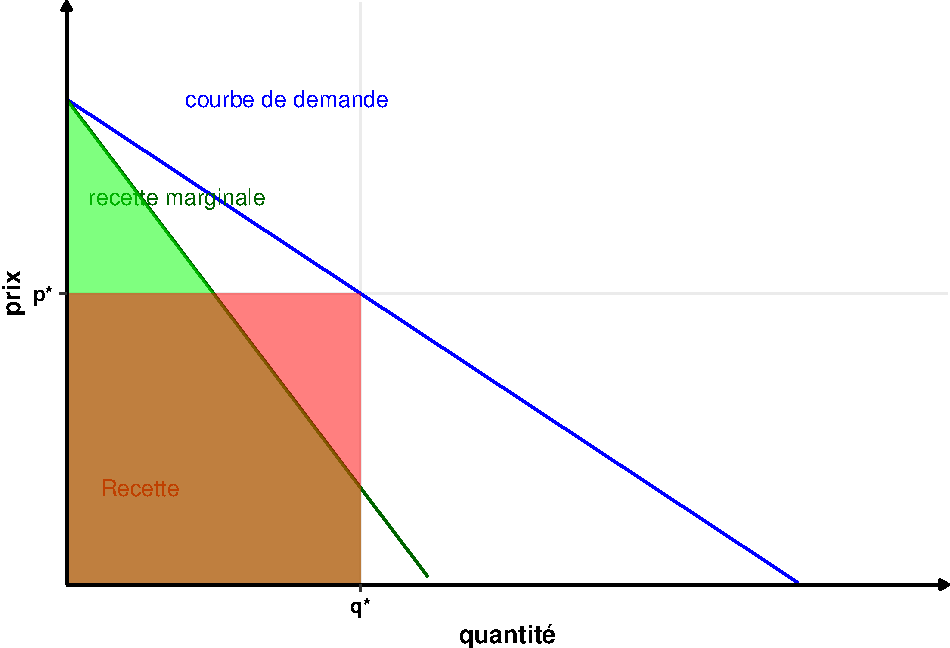
\includegraphics{_main_files/figure-latex/profit-1.pdf}
\caption{\label{fig:profit}Recette maximale.}
\end{figure}

On peut calculer le profit de deux manières :

\begin{enumerate}
\def\labelenumi{\arabic{enumi}.}
\tightlist
\item
  En utilisant l'aire du trapèze vert (intégrale de la recette marginale entre 0 et la quantité produite \(p^*\)) ;
\item
  En utilisant l'aire du rectangle rouge (\(\pi=p^* q^*\)).
\end{enumerate}

Le résultat provient de l'égalité d'aire entre le triangle vert et le triangle rouge.

\hypertarget{duxe9cision-de-production-du-monopole}{%
\section{Décision de production du monopole}\label{duxe9cision-de-production-du-monopole}}

\hypertarget{maximisation-du-profit}{%
\subsection{Maximisation du profit}\label{maximisation-du-profit}}

Comme dans le cas de la CPP, on suppose que le monopole cherche à maximiser son profit \(\pi(q)=R(q)-C(q)\), où \(C(q)\) est la fonction de coût (total) du monopole.\\
Il y a 2 conditions d'optimalités, les conditions de premier (la dérivée du profit à l'optimum est nulle: \(\pi'(q^*)=0\)) et second ordre (la dérivée seconde du profit à l'optimum est strictement négative \(\pi''(q^*)<0\)), ainsi qu'une contrainte, que le profit à l'optimum soit positif (\(\pi(q^*)>0\)).

La condition de premier ordre s'exprime ainsi :
\[
\begin{array}{rcl}
\frac{d\pi(q^*)}{dq} &=&0\\
\Leftrightarrow \frac{dR(q^*)}{dq} - \frac{dC(q^*)}{dq} &=& 0\\
\Leftrightarrow R_m(q^*) &=&C_m(q^*) \label{eq:cpo}
\end{array}
\]

On doit avoir égalité du coût marginal et du revenu marginal à l'optimum.

La condition du second ordre s'exprime ainsi :
\[
\begin{array}{rcl}
\frac{d^2\pi(q^*)}{dq^2} &<&0\\
\Leftrightarrow \frac{dR_m(q^*)}{dq} - \frac{dC_m(q^*)}{dq} &<& 0\\
\Leftrightarrow \frac{dR_m(q^*)}{dq} &<&\frac{dC_m(q^*)}{dq} \label{eq:cso}
\end{array}
\]
La dérivée de la recette marginale doit être inférieure à la dérivée du coût marginal.
Autrement dit, la recette marginale doit croître moins vite que le coût marginal.
Cette condition est en particulier vérifiée si la recette marginale est décroissante et le coût marginal croissant.

Finalement, il faut vérifier que le profit à l'optimum est positif (\(\pi(q^*)>0\)).
Dans le cas contraire, le marché n'existerait tout simplement pas, car le monopole ne voudrait pas produire le bien.

\begin{figure}
\centering
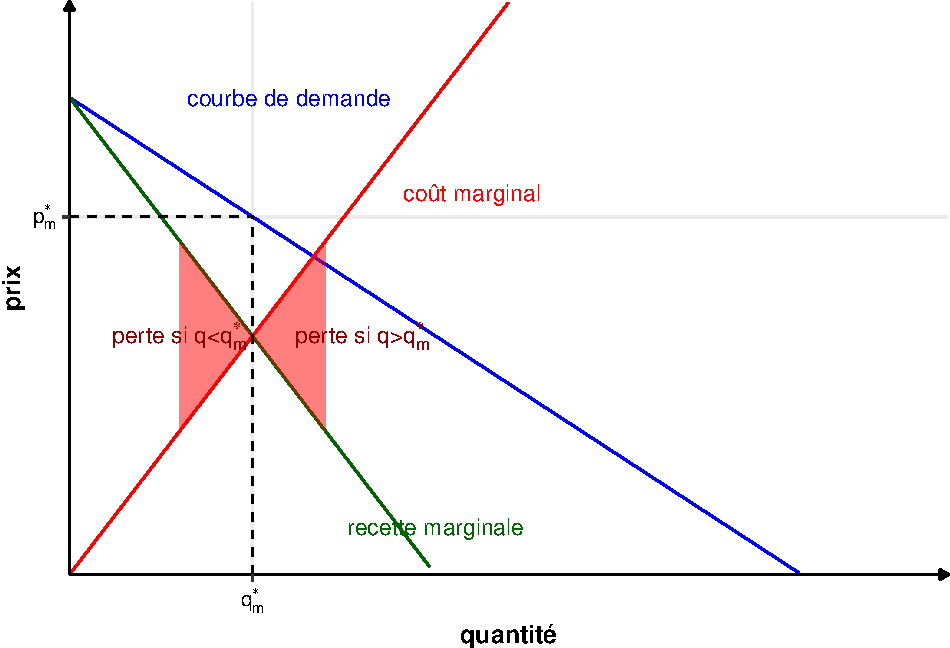
\includegraphics{_main_files/figure-latex/monopoleoptimale-1.pdf}
\caption{\label{fig:monopoleoptimale}Production optimale du monopole.}
\end{figure}

Le prix est lu et obtenu sur la courbe de \textbf{demande}.

\begin{example}[Maximisation du monopole]
Prenons un monopole avec une fonction de coût \(C(q)=50+q^2\).
Le monopole fait face à une demande inverse \(P(q) = 40-q\).

Le coût marginal est :
\[
C_m(q) = \frac{dC(q)}{dq}=2q
\]

La recette totale est :
\[
R(q) = qP(q) = q(40-q) = 40q-q^2
\]
La recette marginale est donc :
\[
R_m(q) = \frac{dR(q)}{dq} = 40 - 2q
\]
Le profit vaut :
\[
\pi(q) = R(q)-C(q)
\]
Conformément à l'équation \eqref{eq:cpo}, il est maximal lorsque :
\[
\begin{array}{rcl}
R_m(q^*) &=&C_m(q^*)\\
\Leftrightarrow 40 -2q &= &2q\\
\Leftrightarrow q^*&=&10
\end{array}
\]
La condition de second ordre de l'équation \eqref{eq:cso} est bien vérifiée, car \(-2<2\).

Le prix de vente vaut :
\[P(q^*) = P(10) = 40-10 = 30\]
La recette vaut 300, le coût 150.
On a donc un profit de \textbf{150}, qui est bien positif.
\end{example}

\begin{figure}
\centering
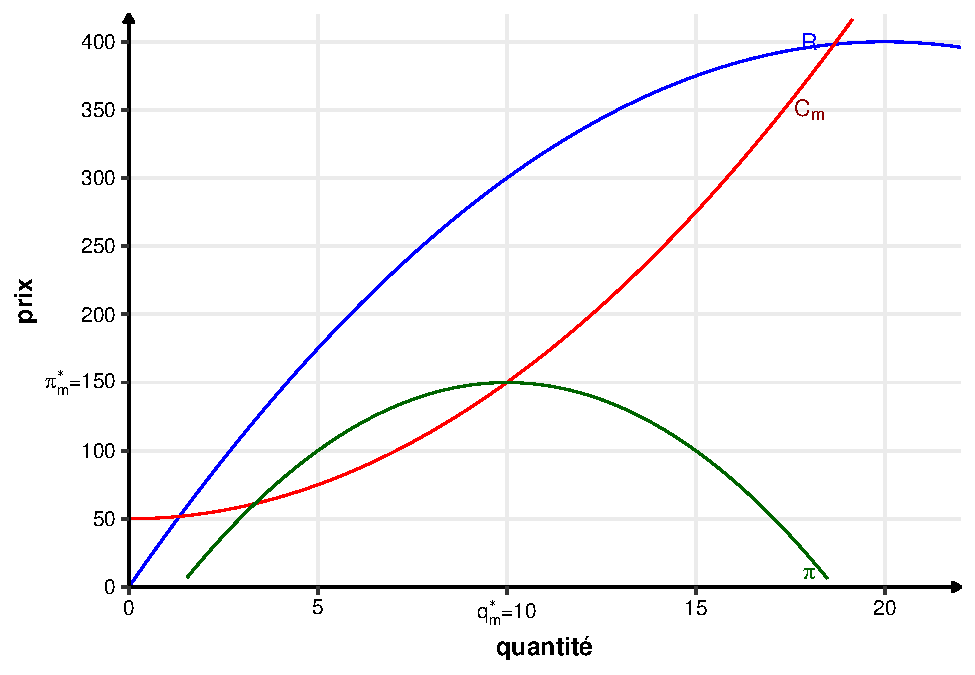
\includegraphics{_main_files/figure-latex/monopolerecette-1.pdf}
\caption{\label{fig:monopolerecette}Recette, coût et profit.}
\end{figure}

\begin{figure}
\centering
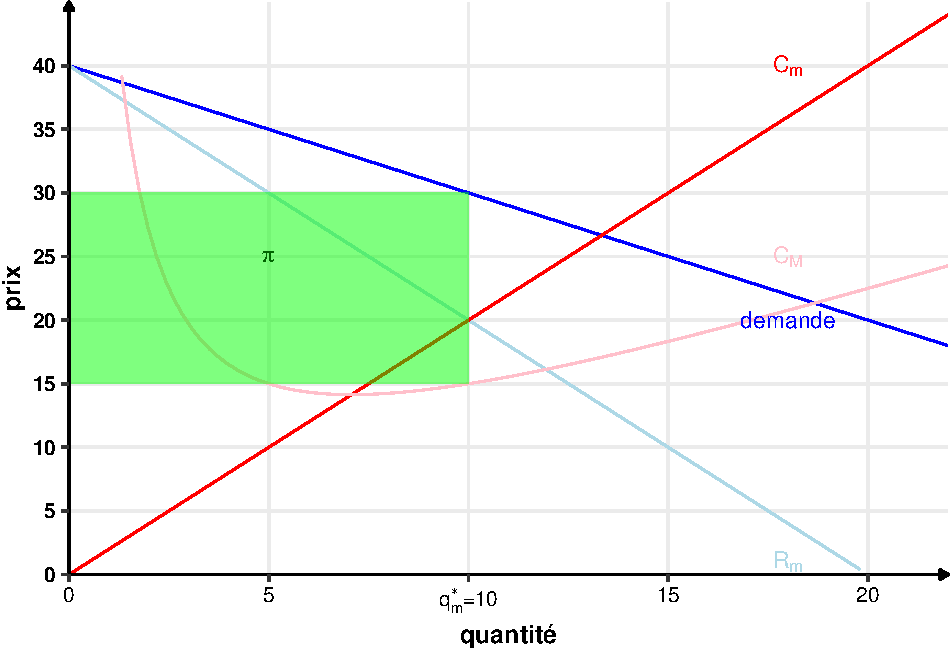
\includegraphics{_main_files/figure-latex/monopoleprofit-1.pdf}
\caption{\label{fig:monopoleprofit}Demande, prix, coûts et profits.}
\end{figure}

\hypertarget{propriuxe9tuxe9s-de-la-solution-de-la-maximisation-du-monopole}{%
\subsection{Propriétés de la solution de la maximisation du monopole}\label{propriuxe9tuxe9s-de-la-solution-de-la-maximisation-du-monopole}}

On avait dans l'équation \eqref{eq:rm} :
\[
R_m(q) = P(q)\left(1 - \frac{1}{|\varepsilon_{q/p}|}\right)\\
\]
Comme à l'optimum, d'après l'équation \eqref{eq:cpo}, on doit avoir \(R_m(q^*)=C_m(q^*)\), on a :
\[
R_m(q^*) = P(q^*)\left(1 - \frac{1}{|\varepsilon_{q/p}(q^*)|}\right) = C_m(q^*) \label{eq:rmcm}
\]
On observe ici un lien avec la solution en CPP.
En effet, en CPP, l'élasticité de la demande au prix est perçue comme infinie, on aura donc bien \(P(q^*) = C_m(q^*)\), la solution obtenue en CPP.
Dès lors que l'élasticité de la demande au prix n'est plus infinie en revanche, on obtient :
\[
 P(q^*)=\frac{C_m(q^*)}{1 - \frac{1}{\left|\varepsilon_{q/p}(q^*)\right|}} > C_m(q^*)
\]

\emph{Question :} Dans quelle zone d'élasticité le monopole va-t-il opérer ?

On voit que si \(\left|\varepsilon_{q/p}(q^*)\right|<1\), c'est-à-dire que si la demande est inélastique, alors \(1 - \frac{1}{\left|\varepsilon_{q/p}(q^*)\right|} <0\), ce qui implique que la recette marginale \(R_m\) est négative, et donc impossible à égaliser avec le coût marginal \(C_m\).\\
On peut voir la réponse d'une autre façon.
Si la pente est inélastique, alors le revenu \(R\) augmente quand la quantité \(q\) baisse.
Le coût total \(C\) baisse aussi quand la quantité baisse.
Le monopole aurait donc tout intérêt à réduire sa production lorsque la demande est inélastique.

\begin{corollary}
Le monopole opère donc nécessairement dans la zone élastique de la courbe de demande : \(\left|\varepsilon_{q/p}(q^*)\right|>1\) .
\end{corollary}

\hypertarget{indice-de-pouvoir-du-monopole}{%
\subsection{Indice de pouvoir du monopole}\label{indice-de-pouvoir-du-monopole}}

La capacité du monopole à vendre à un prix supérieur au coût marginal dépend de la plus ou moins grande élasticité de la demande au prix.
Cela permet de construire un indice du \emph{pouvoir de monopole} à partir de l'élasticité du prix à la demande à l'équilibre.
On a d'après l'équation \eqref{eq:rmcm} :
\[
R_m(q^*) = P(q^*)\left(1 - \frac{1}{|\varepsilon_{q/p}(q^*)|}\right) = C_m(q^*) 
\]
On en déduit :

\[\begin{array}{rl}
& C_m(q^*) = P(q^*) - \frac{P(q^*)}{|\varepsilon_{q/p}(q^*)|}\\
\Leftrightarrow & P(q^*) - C_m(q^*) = \frac{P(q^*)}{|\varepsilon_{q/p}(q^*)|}
\end{array}
\]

\begin{definition}[Indice de Lerner]
\protect\hypertarget{def:Lerner}{}\label{def:Lerner}On définit l'indice de Lerner par :
\[
\frac{1}{|\varepsilon_{q/p}(q^*)|} = \frac{P(q^*) - C_m(q^*)}{P(q^*)} \label{eq:Lerner}
\]
La partie gauche de l'équation est l'indice de Lerner, et la partie droite indique la capacité du monopole à vendre au-dessus de son coût marginal, en pourcentage du prix total.
\end{definition}

On peut construire à partir de l'équation précédente le \emph{markup pricing}.

\begin{definition}[Markup pricing]
\[
P(q^*) =\frac{|\varepsilon_{q/p}(q^*)|}{|\varepsilon_{q/p}(q^*)|-1} C_m(q^*)
\]
\end{definition}

\hypertarget{variation-de-la-demande}{%
\subsection{Variation de la demande}\label{variation-de-la-demande}}

Les décisions de production du monopole et la fixation de son prix dépendent de la demande à laquelle il fait face et du coût marginal.
Le monopole n'a \textbf{pas de courbe d'offre} au sens où il n'y a pas de relation univoque entre prix et quantité produite, à la différence des producteurs en CPP.
En monopole, si la demande change, le monopole s'adapte, soit en changeant sa production, mais pas son prix, ou l'inverse.

\begin{figure}
\centering
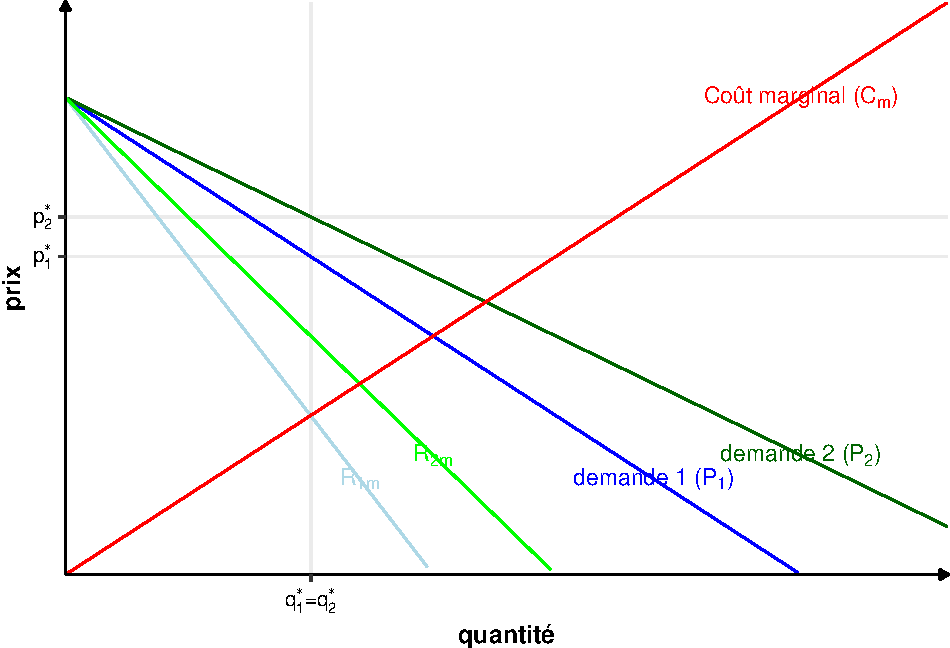
\includegraphics{_main_files/figure-latex/monopolechangementdemande1-1.pdf}
\caption{\label{fig:monopolechangementdemande1}Exemple de réaction du monopole à un changement de demande: changement de prix.}
\end{figure}

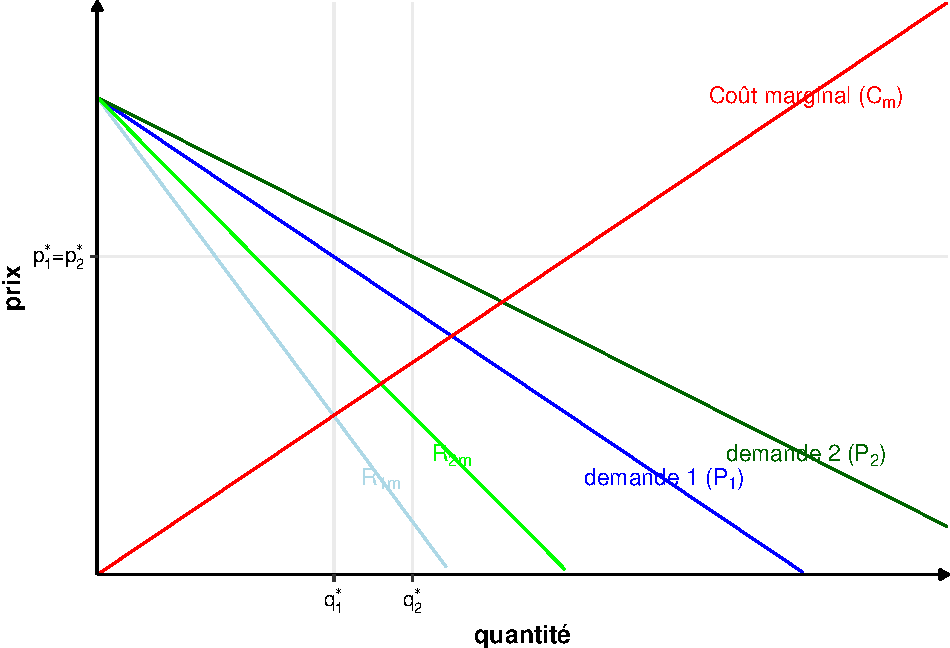
\includegraphics{_main_files/figure-latex/monopolechangementdemande2-1.pdf}
GRAPH avec changement de demandes

En CPP, un changement de demande, si elle implique une changement du prix d'équilibre, entraîne forcément un changement dans la quantité produite par un producteur individuel.

\hypertarget{linefficience-du-monopole}{%
\subsection{L'inefficience du monopole}\label{linefficience-du-monopole}}

La production du monopole est inférieure à la production en CPP, et le prix est supérieur au prix de CPP.

GRAPH avec surplus du monopole

Cela signifie que le surplus du producteur (son profit) est plus élevé en monopole qu'en CPP, et que le surplus des consommateur est plus faible.
Il y a globalement une perte sèche de surplus total.
\textbf{Le monopole est inefficace au sens de Pareto.}
Il existe des consommateurs prêt à acheter à un prix supérieur au coût marginal (dans le triangle de la perte sèche).
Il est donc possible d'avoir une amélioration parétienne qui améliore à la fois la situation des consommateurs et du monopole.
Il suffirait pour cela que le monopole produise une unité supplémentaire du bien à un prix supérieur au coût marginal, sans rien changer d'autre pour obtenir cette amélioration.

\hypertarget{ruxe9gulation-des-monopole}{%
\section{Régulation des monopole}\label{ruxe9gulation-des-monopole}}

Cette partie va traiter de la manière dont un gouvernement peut inciter un monopole à modifier son comportement.

\hypertarget{taxe-unitaire}{%
\subsection{Taxe unitaire}\label{taxe-unitaire}}

Un gouvernement impose une taxe de \(t\) unités monétaire par unité de bien produite.
On a donc :

\[
\pi(q) = R(q) - C(q) -tq
\]
La condition de première ordre de la maximisation du producteur de l'équation \eqref{eq:cpo} devient alors :
\[
\begin{array}{rl}
&\frac{d(R(q)-C(q) -tq)}{dq}(q^*) = 0\\
\Leftrightarrow & R_m(q^*)-C_m(q*) -t = 0\\
\Leftrightarrow & R_m(q^*) = C_m(q^*) + t
\end{array}
\]
Le problème est exactement le même que précédemment, en intégrant la taxe dans le coût marginal.
Pour le monopole, c'est comme si l'état ajoutait un coût \(t\) à chaque unité produite, ce qui est effectivement ce que l'état fait.

GRAPH avec une translation du coût marginal.

Cela entraîne une diminution de la quantité produite et une augmentation du prix.
Le surplus des consommateurs baisse, ainsi que celui du monopole.

Une vue \textbf{alternative} à l'augmentation du coût marginal est de considérer que la taxe diminue la recette marginale de \(t\) :
\[
 R_m(q^*) -t = C_m(q^*)
\]

GRAPH avec diminution de la recette marginale.

Si le gouvernement utilise une taxe négative (= une subvention), alors le gouvernement peut augmenter la production et de diminuer le prix.

\hypertarget{taxe-forfaitaire}{%
\subsection{Taxe forfaitaire}\label{taxe-forfaitaire}}

Avec une taxe forfaitaire, l'état prélève un montant \(T\) indépendant de la quantité produite sur le profit du producteur.
\[
\pi(q) = R(q) - C(q) -T
\]
La condition du premier ordre de l'équation \eqref{eq:cpo} devient alors :
\[
\begin{array}{rl}
& \frac{d(R(q)-C(q) -T)}{dq}(q^*) = 0\\
\Leftrightarrow & R_m(q^*)-C_m(q*) = 0\\
\Leftrightarrow & R_m(q^*) = C_m(q^*)
\end{array}
\]
On retrouve exactement la même condition d'optimalité qu'en l'absence de taxe.
Si elle n'est pas trop élevée, une taxe forfaitaire n'a \emph{aucune} influence sur la quantité produite et prix.
Si la taxe forfaitaire est très élevée, supérieure au profit \(R(q^*) - C(q^*) <T\), le monopole préfère ne rien produire et le surplus social est nul.

On peut donc envisager de combiner une subvention unitaire au monopole combinée à une taxe forfaitaire pour augmenter le surplus total.

\hypertarget{impuxf4t-sur-profit}{%
\subsection{Impôt sur profit}\label{impuxf4t-sur-profit}}

Au lieu de taxer chaque unité produite, on peut taxe le niveau de profit à un taux \(t\).
Le profit devient alors
\[
\pi(q) = R(q) - C(q) -t( R(q) - C(q)) = (1-t)(R(q) - C(q))
\]
La condition du premier ordre de l'équation \eqref{eq:cpo} devient alors :
\[
\begin{array}{rl}
&\frac{d((1-t)(R(q)-C(q)))}{dq}(q^*) = 0\\
\Leftrightarrow & (1-t)(R_m(q^*)-C_m(q*)) = 0\\
\Leftrightarrow & R_m(q^*) = C_m(q^*)
\end{array}
\]

Comme pour la taxe forfaitaire, le comportement du monopole n'est pas modifié par une taxe sur le profit.
On peut donc aussi envisager une subvention à la production et une taxe proportionnelle sur le profit.

\hypertarget{fixation-dun-prix-maximum}{%
\subsection{Fixation d'un prix maximum}\label{fixation-dun-prix-maximum}}

Le gouvernement interdit de vendre au-dessus d'une prix maximum \(p^{max}\)

Le gouvernement modifie ainsi la demande perçue par le producteur.

GRAPH

Si le prix maximum est inférieur au prix de concurrence pure et parfaite, les quantités produites peuvent devenir sous-optimale.
Le gouvernement peux maximiser le surplus social en prenant le prix concurrentiel comme prix maximum.\\
\emph{Rappel :} En CPP, on obtient le prix à l'aide de la courbe de coût marginal.
L'équilibre est au moment a lieu quand le coût marginal est la demande se croisent.

GRAPH

Avec un prix maximum égal au prix de concurrence pure et parfaite, le revenu marginal comme la courbe de coût marginal au point d'équilibre de la concurrence pure et parfaite.

Globalement, si le prix maximal est entre le prix de monopole et le prix de concurrence pure et parfaite, alors la quantité produite augment quand le prix maximal diminue.
Si au contraire le prix maximal est inférieur au prix de CPP (et donc de monopole), alors la quantité produite diminue quand le prix maximal augmente.

\hypertarget{le-monopole-naturel}{%
\section{Le monopole naturel}\label{le-monopole-naturel}}

Une situation de monopole naturel émerge à cause d'une structure particulière de la technologie de production et des coûts, plutôt qu'à cause d'une disposition légale.

\begin{definition}[Monopole naturel]
Un monopole naturel émerge en présence d'une technologie dotée de rendements d'échelles \emph{croissants} dans la zone de production optimale.
\end{definition}

Les rendements d'échelles sont croissants lorsque la technologie de production \(f\) est telle que :
\[
f(\lambda z_1, \lambda z_2, ...\lambda z_n) > \lambda f(z_1,z_2, ..., z_n)
\]
où les \(z_i\) sont les facteurs de productions.
En mots : une entreprise utilisant \(\lambda\) fois plus de facteurs de productions qu'une petite entreprise produit plus que \(\lambda\) petites entreprises réunies.

En général, un monopole naturel émerge à cause de coûts fixes élevés.
Par exemple, lorsqu'il faut investir dans un réseau (ferrés, téléphone, électricité, etc).

Une conséquence des économies d'échelles est que le coût moyen est décroissant :
\[
C_M(f(\lambda z)) =\frac{\lambda z\cdot w_z}{f(\lambda z)} < C_M(\lambda f(z)) = \frac{\lambda z\cdot w_z}{\lambda f(z)}
\]
car \(f(\lambda z)>\lambda f(z)\)
Cela signifie qu'une seule entreprise qui produit \(f(\lambda z)\) est plus efficace que \(\lambda\) entreprises qui produisent \(\lambda f(z)\).

De manière générale, il y a presque toujours une zone où le coût moyen est décroissant, mais elle est rarement très étendue.

GRAPH avec zone d'économie d'échelle.

\emph{Rappel :} Lorsque le coût moyen est décroissant, c'est que le coût marginal est inférieur au coût moyen.
\[
CM(q) = \frac{C(q)}{q}
\]
\[
CM'(q) =\frac{C'(q)q-C(q)}{q^2} = \frac{C_m(q)-C_M(q)}{q}
\]
Or \(CM'(q)<0\), comme le coût marginal est décroissant.
On en déduit donc que
\[
C_m(q)-C_M(q)< 0 \Leftrightarrow C_m(q)<C_M(q)
\]

\textbf{Question :} Que se passe-t-il quand la fonction de demande inverse coupe la courbe de coût marginal dans la partie ou le coût marginal est inférieur au coût moyen (où \(C_m<C_M\)) ?

GRAPH avec les courbes de coût moyen et coût marginaux.

Si on impose une tarification au coût marginal, alors le monopole fait des pertes, car le prix est inférieur au coût moyen.
La régulation ``optimale'' généralement utilisée impose \emph{un prix au coût moyen} et une obligation de satisfaire toute la demande.
Le monopole fait alors un profit nul.

Une solution alternative est un prix égal au coût moyen assorti de subventions pour couvrir les pertes.

\hypertarget{le-monopole-discriminant}{%
\section{Le monopole discriminant}\label{le-monopole-discriminant}}

Un monopole discriminant pratique un prix différent pour chaque (groupe de) consommateur.
Pour cela, il doit pouvoir identifier l'appartenance de chaque consommateur à un groupe et les marchés entre les consommateurs doivent être hermétiques.
En particulier, il ne faut pas qu'un consommateur puisse revendre son unité de produit à un autre consommateur.

Il existe 3 types de discriminations par les prix, les discrimination du premier, deuxième et troisième degrés.
On ne traitera que les discriminations du premier et troisième degré.

\hypertarget{discrimination-au-premier-degruxe9-discrimination-parfaite}{%
\subsection{Discrimination au premier degré (discrimination parfaite)}\label{discrimination-au-premier-degruxe9-discrimination-parfaite}}

Dans une discrimination parfaite, le monopole connaît la valorisation (prix de réserve) de chaque individu et lui fait payer le prix maximum qu'il est prêt à payer (son prix de réserve donc).
Le consommateur ne retient alors aucun surplus, la \emph{totalité} du surplus est capturé par le producteur.

\emph{Question :} Quel va être le niveau de production du monopole ?

Comme le monopole fait payer chaque unité à la valorisation du consommateur, la première unité est vendue au prix P(1), la deuxième au prix P(2), etc.
La recette totale est donc :
\[
R(q) = \int_0^q P(x) dx
\]
Notons le coût total \(C(q)\).
Le profit est :
\[
\pi(q) = R(q) - C(q) = \int_0^q P(x) dx -C(q)
\]
La condition du premier ordre s'écrit donc :
\[
\begin{array}{rl}
&\frac{d\pi(q^*)}{dq} = 0\\
\Leftrightarrow & \frac{d\int_0^{q^*} P(x) dx -C(q^*)}{dq} = 0\\
\Leftrightarrow & P(q^*) - C_m(q^*) = 0\\
\Leftrightarrow & P(q^*) = C_m(q^*)
\end{array}
\]
La recette marginale est ici confondue avec la courbe de demande.
L'optimum se trouve donc au point où la courbe de coût marginal coupe la courbe de demande (inverse).
C'est la même condition qu'en CPP.
Le monopole parfaitement discriminant produit donc la quantité de concurrence pure et parfaite.
Le prix de la dernière unité vendue par le monopole est égal au prix de la concurrence pure et parfaite, même si les prix des autres unités vendues sont supérieur au prix de la CPP.

GRAPH avec discrimination parfaite

La situation de discrimination parfaite est un optimum de Pareto.
En effet, le surplus social est maximal (mais capturé entièrement par le monopole).

En pratique, il est très difficile de faire de la discrimination parfaite.
Les entreprises essaient de s'en approcher le plus possible.

Un exemple existe, lors d'une vente de bons du trésors des Etats-Unis.
Chaque ménage intéressé soumettait une offre (prix, quantité) au gouvernement.
Le gouvernement triait les offres par ordre décroissant de prix et les satisfait jusqu'à épuisement des bons à vendre.

\hypertarget{discrimination-du-deuxiuxe8me-degruxe9}{%
\subsection{Discrimination du deuxième degré}\label{discrimination-du-deuxiuxe8me-degruxe9}}

\begin{definition}[Discrimination du deuxième degré]
La discrimination du deuxième degré a lieu lorsque les prix de ventes dépendent des quantités achetées.
\end{definition}

Par exemple, si les 10 premières unités vendues le sont à 5€, et les suivantes à 2€.
Les prix de ventes sont nécessairement \emph{décroissants} avec la quantité vendue.

GRAPH avec 3 seuils de quantité.

Le monopole ajuste les quantités seuil afin de maximiser son profit.
Il y a un nombre fini de seuils de dégressivité.
Plus il y a de seuils, plus on s'approche d'un situation de discrimination parfaite.

\hypertarget{discrimination-du-troisiuxe8me-degruxe9}{%
\subsection{Discrimination du troisième degré}\label{discrimination-du-troisiuxe8me-degruxe9}}

A faire si le temps le permet.

Il s'agit de faire payer un prix différent à chaque groupe de consommateur, en fonction des caractéristiques de leurs fonctions de demande.
Tous les membres d'un groupe payent donc le même prix, contrairement à la discrimination au premier degré.
Les groupes sont en général caractérisés par des propensions à payer différentes.
Il s'agit d'une segmentation des consommateurs.

\begin{example}[Discrimination au troisième degré]
Les tarifs jeunes de la SNCF, les tarifs familles.
Il est important de pouvoir identifier les groupes.
\end{example}

\emph{Question :} Comment répartir la production entre les différents groupes ?

\begin{enumerate}
\def\labelenumi{\arabic{enumi}.}
\tightlist
\item
  Quelle production totale ?
\item
  Quelle répartition ?
\end{enumerate}

\emph{Méthode :} On résout d'abord 2 en supposant que 1 est déjà résolu.
On obtient alors la répartition en fonction de la production totale.
Puis ou résout 1 à l'aide de la solution de 2.

On modélise le problème de la manière suivante :

\begin{itemize}
\tightlist
\item
  2 groupes A et B;
\item
  Avec des fonctions de demande inverses \(P_A(q_A)\) et \(P_B(q_B)\);
\item
  Une quantité \(q\) totale a été produite, qu'il faut répartir entre les 2 groupes : \(q=q_A+q_B\)
\end{itemize}

Le problème du monopole s'écrit :
\[
\max_{q_A, q_B} \pi(q_A, q_B) = q_AP_A(q_A) + q_BP_B(q_B) -C(q)
\]
La quantité totale \(q\) est fixée, donc le coût total l'est aussi et peut être supprimé du problème de maximisation.
On cherche donc juste à maximiser la recette totale :
\[
\max_{q_A, q_B} q_AP_A(q_A) + q_BP_B(q_B) 
\]
Avec \(q=q_A+q_B\), donc \(q_B=q-q_A\), le problème devient :
\[
\begin{array}{rl}
&\max_{q_A, 0\leq q_A\leq q} q_AP_A(q_A) + (q-q_A)P_B(q-q_A) \\
\Leftrightarrow &\max_{q_A, 0\leq q_A\leq q} R_A(q_A) + R_B(q-q_A) 
\end{array}
\]
La condition du premier ordre s'écrit :
\[
\begin{array}{rl}
&\frac{dR_A(q_A) + R_B(q-q_A) }{dq_A} = 0\\
\Leftrightarrow & R_{mA}(q_A) - R_{mB}(q-q_A) = 0\\
\Leftrightarrow & R_{mA}(q_A) = R_{mB}(q_B) 
\label{eq:cpo3e}
\end{array}
\]
L'équation \eqref{eq:cpo3e} nous dit que le monopole réparti la quantité totale produite de manière égaliser les recettes marginales entre les deux groupes.

Intuitivement, si la recette marginale issue du groupe A est supérieure à celle issue du groupe B (\(R_{mA}(q_A) > R_{mB}(q_B)\)), alors en diminuant la quantité \(q_B\) dans le groupe B et en la transférant au groupe A, le monopole perd \(R_{mB}(q_B)\) et gagne \(R_{mA}(q_A)\), donc la recette totale augmente et le profit aussi.
Inversement dans le cas opposé.
Il n'est donc pas intéressant de transférer la production d'un groupe vers un autre lorsque \(R_{mA}(q_A) = R_{mB}(q_B)\) (et seulement dans ce cas).

Maintenant que la répartition est résolue, il faut trouver la quantité totale produite.
Le problème devient maintenant :
\[
\max_{q_A, q_B} \pi(q_A, q_B) = q_AP_A(q_A) + q_BP_B(q_B) -C(q_A+q_B)
\]
La condition du premier ordre s'obtient maintenant en dérivant suivant \(q_A\) et \(q_B\) séparément :
\[
\begin{array}{rcl}
\frac{\partial\pi(q_A, q_B)}{\partial q_A} = 0&\Leftrightarrow& R_{mA}(q_A^*) = C_m(q_A^*+q_B^*)\\
\frac{\partial\pi(q_A, q_B)}{\partial q_B} = 0&\Leftrightarrow& R_{mB}(q_B^*) = C_m(q_A^*+q_B^*)\\
\end{array}
\]
Le monopole doit faire en sorte que le coût marginal de sa production totale soit égale à la recette marginale sur chacun des marchés.

\emph{Intuition :}
Le monopole doit égaliser la recette marginale sur les deux marchés.
Or le coût marginal dépend de la quantité \emph{totale} produite, pas de la répartition entre les marchés.
Si on est dans la situation telle que \(C_m(q)<R_{mA}(q_A)\), alors il y a la possibilité de faire du profit sur le marché A (et le marché B par conséquent).
Inversement, si \(C_m(q)>R_{mA}(q_A)\), alors le monopole fait des pertes.

NB: On utilise bien \(C_m(q_A+q_B)\) et non \(C_m(q_A)\) ou \(C_m(q_B)\) car c'est bien la variation du coût total lorsqu'on augmente ``un peu'' \(q_A\) et \(q_B\) reste fixe.

D'après l'équation \eqref{eq:rm}, on peut écrire :
\[
\begin{array}{crcl}
&R_{mA}(q_A^*) &=& R_{mB}(q_B^*)\\
\Leftrightarrow & P_A(q_A^*)\left(1-\frac{1}{\left|\varepsilon_{q/p_A}\right|}\right) & = & P_B(q_B^*)\left(1-\frac{1}{\left|\varepsilon_{q/p_B}\right|}\right)
\end{array}
\]
Sans perte de généralité, on peut supposer que \(P_A(q_A^*)> P_B(q_B^*)\).
On obtient alors que :
\[
1-\frac{1}{\left|\varepsilon_{q/p_A}\right|} <1-\frac{1}{\left|\varepsilon_{q/p_B}\right|}
\]
Autrement dit
\[
\left|\varepsilon_{q/p_B}\right|>\left|\varepsilon_{q/p_A}\right|
\]
Le prix est donc plus faible pour le groupe où l'élasticité prix de la demande est plus élevée.
Le prix est plus élevé pour le groupe avec l'élasticité la plus faible, les moins réactifs au prix.

\begin{example}
Les tarifs ``professionnels'' dans les transports (avion, train, etc).
Les professionnels sont moins sensibles au prix car leurs dates de voyage sont moins flexibles que celles des particuliers.
Leur élasticité prix est donc plus faible et leurs prix plus élevés.
\end{example}

Des fonctions de demande inverse différentes associées à des élasticités prix de la demande différente aboutissent à des prix différents.

\hypertarget{oligopoles}{%
\chapter{Oligopoles}\label{oligopoles}}

\hypertarget{introduction}{%
\section{Introduction}\label{introduction}}

On a vu jusqu'à présent deux cas extrêmes :

\begin{itemize}
\tightlist
\item
  La concurrence pure et parfaite :
  il y a une infinité d'entreprise infinitésimales sur un marché donné.
\item
  Le monopole : il y a une seule entreprise sur un marché donné.
\end{itemize}

Dans les deux cas, l'entreprise ou les entreprises n'ont pas à se préoccuper des autres entreprises.
Dans le cas du monopole, parce qu'il n'y en a pas.
Dans le cas de la CPP, l'entreprise observe le prix du marché et prend sa décision en fonction de ce prix, et uniquement de ce prix.
Les actions des autres entreprises ne l'influence pas.

On considère maintenant la situation où il n'y a plus une seule ou une infinité d'entreprises, mais plusieurs, qui sont en situation d'\emph{interactions stratégiques}.
Les décisions de chaque acteur dépend des décisions des autres acteurs (ou des anticipations de ces décisions).\\
On parle de \emph{duopole} dans le cas où le marché compte deux entreprises et d'\emph{oligopole} dans le cas où il compte plus que deux entreprises.\\
Les entreprises peuvent se faire concurrence de différentes manières :

\begin{itemize}
\tightlist
\item
  En quantité, concurrence dite à la \emph{Cournot} ;
\item
  En prix, concurrence à la \emph{Bertrand} ;
\item
  En prenant une situation de leader ou de follower, à la \emph{Stackelberg} ;
\item
  En format une entente, dans un \emph{cartel} ;
\item
  Dans une concurrence spatiale, à la \emph{Hotelling}.
\end{itemize}

Nous verrons dans ce cours les concurrences à la Cournot et à la Stackelberg, ainsi que les cartels.

\hypertarget{duopole-uxe0-la-cournot}{%
\section{Duopole à la Cournot}\label{duopole-uxe0-la-cournot}}

\hypertarget{introduction-1}{%
\subsection{Introduction}\label{introduction-1}}

On considère deux entreprises sur le même marché qui doivent choisir les quantités à produire, sans connaître la quantité choisie par l'autre (= décision simultanée).\footnote{Même marché : bien unique et prix unique.}
Le prix est déterminé par la quantité \emph{totale} produite par les deux entreprises et la fonction de demande sur le marché.

Chaque entreprise est caractérisée par :

\begin{itemize}
\tightlist
\item
  Entreprise 1 : quantité \(q_1\) produite avec un coût \(C_1(q_1)\) ;
\item
  Entreprise 2 : quantité \(q_2\) produite avec un coût \(C_2(q_2)\).
\end{itemize}

Les fonctions de coût sont \textbf{différentes} entre les deux entreprises, contrairement au cas du monopole discriminant au troisème degré, où l'on considérait \(C(q_1+q_2)\).

La fonction de demande inverse sur le marché est \(P(q_1+q_2)\).
C'est différent du monopole discriminant où il y avait une fonction de demande par segment.

On a donc les fonctions de profit:
\[
\begin{array}{rcl}
\pi_1(q_1, q_2) &=& P(q_1+q_2)\cdot q_1-C_1(q_1)\\
\pi_2(q_1, q_2) &=& P(q_1+q_2)\cdot q_2-C_2(q_2)
\end{array}
\]
L'action d'une entreprise a des conséquences sur le profit réalisé par l'autre entreprise, même si celle-ci ne fait rien.
En particulier, si \(q_1\) augmente, alors le prix du marché diminue, au travers de la fonction de demande inverse \(P\), et donc le profit de l'entreprise 2 \(\pi_2\) diminue, et réciproquement si \(q_2\) augmente.
Il y a donc un conflit d'intérêt entre les producteurs.
Chaque entreprise doit anticiper l'action de l'autre et réagir à cette anticipation le mieux possible.

\emph{Question :} Peut-il y avoir un équilibre dans cette situation ?

\hypertarget{formalisation-du-probluxe8me}{%
\subsection{Formalisation du problème}\label{formalisation-du-probluxe8me}}

\hypertarget{expression-des-profits}{%
\subsubsection{Expression des profits}\label{expression-des-profits}}

On a des profits :
\[
\begin{array}{rcl}
\pi_1(q_1, q_2) &=& P(q_1+q_2)\cdot q_1-C_1(q_1)\\
\pi_2(q_1, q_2) &=& P(q_1+q_2)\cdot q_2-C_2(q_2)
\end{array}
\label{eq:profitcournot}
\]

Supposons que l'entreprise 1 \emph{croit} que l'entreprise 2 va produire \(q_2^a\).
Quelle est sa production optimale ?
Son problème est :
\[
\max_{q_1} \pi_1(q_1, q_2^a) =  q_1P(q_1+q_2^a)-C_1(q_1)
\]
On peut déduire de ce problème d'optimisation la \emph{fonction de réaction} \(q_1(q_2^a)=f_1(q_2^a)\) qui maximise \(\pi_1(q_1)\) en fonction de la production anticipée \(q_2^a\) de l'entreprise 2.\footnote{La fonction de réaction est parfois aussi connue sous le nom de \emph{fonction de meilleure réponse}.}
La fonction de réaction \(f_1(q_2^a)\) donne la valeur de \(q_1\) qui maximise le profit quand l'entreprise 2 produit \(q_2^a\).

De la même manière, l'entreprise 2 cherche à maximiser \(\pi_2\) en fonction de la production anticipée \(q_1^a\) de l'entreprise 1.
Son programme est :
\[
\max_{q_2} \pi_2(q_1^a, q_2) =  q_1P(q_1^a+q_2)-C_2(q_2)
\]
Elle aura également une fonction de réaction \(q_2(q_1^a)=f_2(q_1^a)\).

\hypertarget{forme-des-fonctions-de-ruxe9action}{%
\subsubsection{Forme des fonctions de réaction}\label{forme-des-fonctions-de-ruxe9action}}

Si l'entreprise \(i\) pense que l'entreprise \(j\) ne va rien produire, alors elle se trouve dans une situation de monopole et se comporte comme tel.
Elle produit de manière à égaliser coût marginal et recette marginale (\(R_{im}=C_{im}\)).

Si l'entreprise \(i\) pense que l'entreprise \(j\) va produire \(q_j^a>0\), alors elle est en monopole sur le \textbf{reste} de la demande.
Cette dernière correspond à la demande totale décalée de \(q_j^a>0\) vers la gauche.
Le croisement entre recette marginale et coût marginal se fait donc à un niveau plus faible qu'auparavant.

Plus l'entreprise \(i\) pense que l'entreprise \(j\) va produire une grande quantité, plus elle aura intérêt à réduire son offre.
\(q_i\) est décroissante en \(q_j^a\)

GRAPH avec la fonction de demande translatée.

\hypertarget{caractuxe9risation-de-luxe9quilibre}{%
\subsubsection{Caractérisation de l'équilibre}\label{caractuxe9risation-de-luxe9quilibre}}

Un équilibre \((q_1^a, q_2^a)\) doit être tel qu'aucune des deux entreprises n'ait intérêt à dévier unilatéralement :
\[
\begin{array}{rcl}
\pi_1(q_1^a, q_2^a) &\geq& \pi_1(q_1, q_2^a)\quad \forall q_1\\
\pi_2(q_1^a, q_2^a) &\geq& \pi_2(q_1^a, q_2)\quad \forall q_2
\end{array}
\]
Aux points \(q_1^a\) et \(q_2^a\), aucune entreprise n'a intérêt à dévier unilatéralement de l'équilibre.
Les décisions prises sont alors mutuellement compatibles.
Chaque entreprise donne sa meilleure réponse à la meilleure réponse de l'autre.
C'est ce qu'on appelle un \textbf{équilibre de Nash} : un équilibre où personne n'a intérêt à dévier unilatéralement.

Dans le cas du duopole à la Cournot, chaque entreprise doit choisir la quantité qui maximise son profit étant donné le choix de l'autre entreprise.
Chaque entreprise est donc sur sa fonction de réaction.
L'équilibre est donc à l'intersection des fonctions de réactions des deux entreprises :
\[
\begin{array}{rcl}
q_1^a&=&f_1(q_2^a)\\
q_2^a&=&f_2(q_1^a)
\end{array}
\]

GRAPH avec une situation d'équilibre.

L'équilibre n'est pas nécessairement stable.
La stabilité dépend de la pente des fonctions de réactions.

GRAPH avec équilibre instable

\hypertarget{exemple}{%
\subsection{Exemple}\label{exemple}}

\hypertarget{donnuxe9es-du-probluxe8me}{%
\subsubsection{Données du problème}\label{donnuxe9es-du-probluxe8me}}

Prenons les fonctions suivantes :

\[
\begin{array}{l}
P(q_1+q_2) = a - b(q_1+q_2)\\
C_1(q_1) = cq^2_1 \\
C_2(q_2) = cq^2_2 \\
\end{array}
\]

\hypertarget{profits}{%
\subsubsection{Profits}\label{profits}}

On en déduit les profits :

\[
\begin{array}{rcl}
\pi_1(q_1, q_2) &=& \left(a-b(q_1+q_2)\right)q_1-cq_1^2\\
\pi_2(q_1, q_2) &=& \left(a-b(q_1+q_2)\right)q_2-cq_2^2
\end{array}
\]

\hypertarget{fonctions-de-ruxe9action}{%
\subsubsection{Fonctions de réaction}\label{fonctions-de-ruxe9action}}

Calculons la fonction de réaction de l'entreprise 1.
Son profit est :
\[
\pi_1(q_1, q_2^a) = aq_1-bq_1^2-bq_2^aq_1-cq_1^2 = (a-bq_2^a)q_1-(b+c)q_1^2
\]

La condition du premier ordre suivant \(q_1\) s'écrit (ici \(q_2^a\) est considéré comme une donnée par l'entreprise 1) :

\[
\begin{array}{crcl}
&\frac{\partial \pi_1}{\partial q_1}&=&0\\
\Leftrightarrow & (a-bq_2^a)-2(b+c)q_1^* &=& 0\\
\Leftrightarrow & q_1^* &=& \frac{(a-bq_2^a)}{2(b+c)}
\label{eq:FR1}
\end{array}
\]

On calcule de la même manière (i.e., en utilisant la condition du premier ordre sur les profits de l'entreprise 2) la fonction de réaction de l'entreprise 2 et on obtient par symétrie du problème une légère réécriture de l'équation \eqref{eq:FR1}:

\[
q_2^* = \frac{(a-bq_1^a)}{2(b+c)}
\]

La symétrie du problème provient du fait que les deux entreprises ont exactement la même fonction de coût.
Ce \emph{n'est pas le cas en général}.
Si dans un problème les fonctions de coût sont identiques, alors vous pouvez faire les calculs pour une seule entreprise et déduire simplement les résultats pour la seconde.

\hypertarget{equilibre-de-cournot}{%
\subsubsection{Equilibre de Cournot}\label{equilibre-de-cournot}}

Quel est alors l'équilibre de Cournot ?

On doit avoir :
\[
\begin{array}{rcl}
f_1(q_2^*) &=& q_1^*\\
f_2(q_1^*) &=& q_2^*\\
\end{array}
\]
Autrement dit :
\[
\begin{array}{rcl}
q_1^* &=& \frac{(a-bq_2^*)}{2(b+c)} \\
q_2^* &=&\frac{(a-bq_1^*)}{2(b+c)}\\
\end{array}
\]
On résout le système et on obtient :
\[
q_1^*=q_2^* = \frac{a}{3b+2c}
\]

\hypertarget{une-intuition-graphique-les-courbes-disoprofit}{%
\subsection{Une intuition graphique : les courbes d'isoprofit}\label{une-intuition-graphique-les-courbes-disoprofit}}

On peut aussi aborder le problème à l'aide d'une intuition graphique.
Il s'agit de tracer les courbes d'\emph{isoprofit} des entreprises.

\begin{definition}[Courbe d'isoprofit]
Les courbes d'isoprofit est l'ensemble des couples de quantités \((q_1, q_2)\) qui permettent à une entreprise d'atteindre un niveau de profit donné.
\end{definition}

Reprenons l'expression générale des profits de l'équation \eqref{eq:profitcournot}.
\[
\begin{array}{rcl}
\pi_1(q_1, q_2) &=& q_1P(q_1+q_2)-C_1(q_1)\\
\pi_2(q_1, q_2) &=& q_2P(q_1+q_2) -C_2(q_2)
\end{array}
\]
La courbe d'isoprofit pour une valeur \(\pi_1\) \textbf{donnée et fixe} est :
\[
\pi_1 = q_1P(q_1+q_2)-C_1(q_1)
\]
L'équation ci-dessus définit implicitement une fonction \(q_1=I_\pi(q_1, \pi_1)\) qui permet de représenter la courbe d'isoprofit dans un graphique \((q_1,q_2)\), tout comme la fonction de réaction définit une fonction courbe \(q_2(q_1)\) pour l'entreprise 1.
La courbe de la fonction de réaction de 1 coupe la courbe d'isoprofit de 1 en son maximum.

\begin{verbatim}
## Scale for 'x' is already present. Adding another scale for 'x', which will
## replace the existing scale.
\end{verbatim}

\begin{figure}
\centering
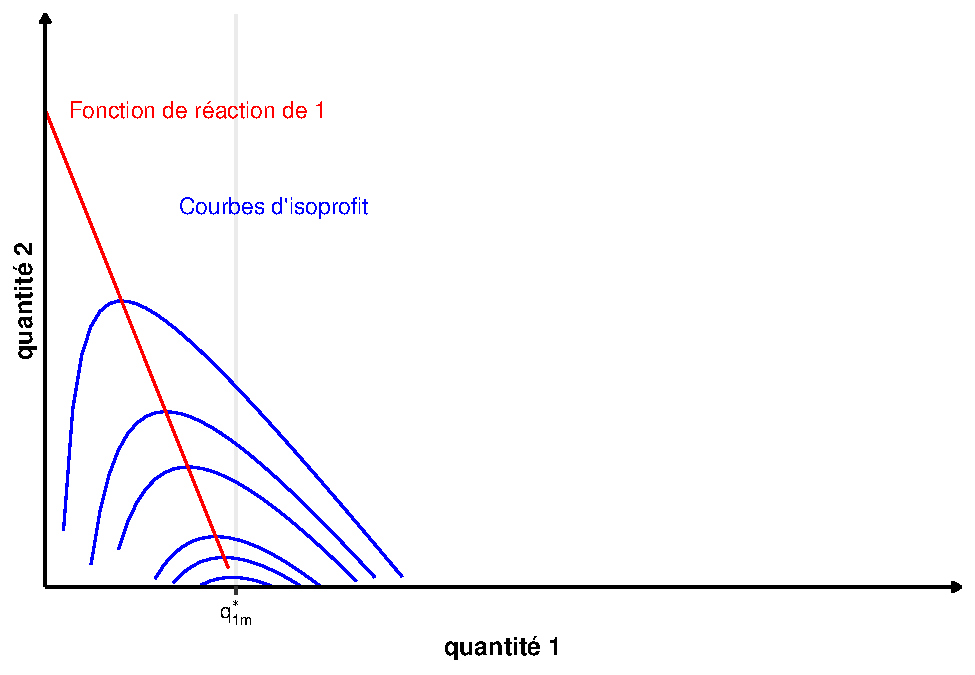
\includegraphics{_main_files/figure-latex/isoprofit1-1.pdf}
\caption{\label{fig:isoprofit1}Courbes d'isoprofit et fonction de réaction de l'entreprise 1}
\end{figure}

Sur la figure \ref{fig:isoprofit1}, le profit est croissant en descendant vers le bas sur les courbes d'isoprofit, autrement dit, les courbes d'isoprofit les plus basses représentent les profits les plus élevés.
Le maximum du profit est atteint lorsque l'entreprise 1 est en monopole.
La quantité produite est alors \(q_m^*\) est le profit \(\pi_m^*\).

\begin{verbatim}
## Scale for 'x' is already present. Adding another scale for 'x', which will
## replace the existing scale.
\end{verbatim}

\begin{figure}
\centering
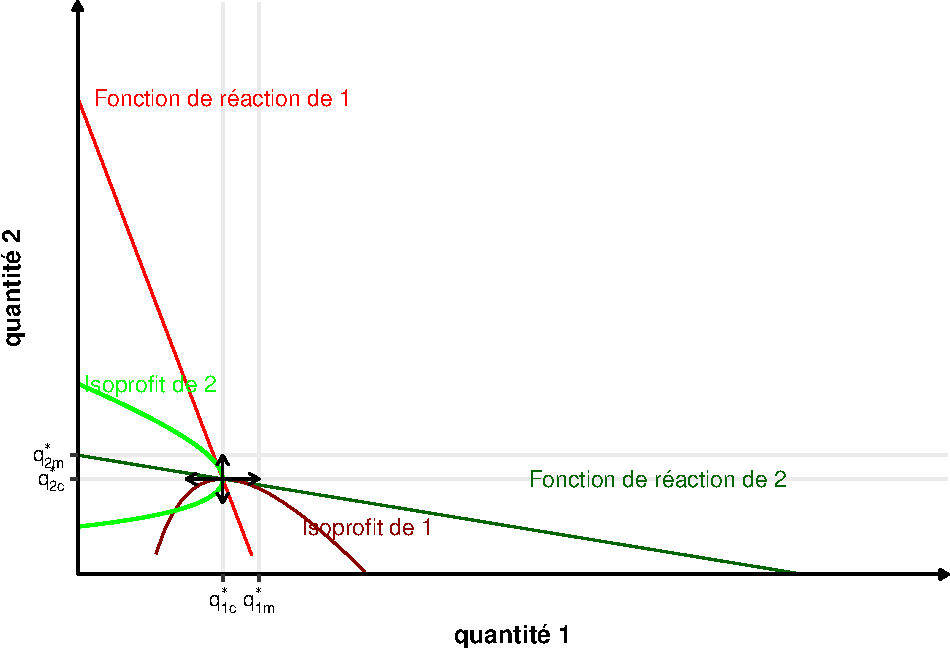
\includegraphics{_main_files/figure-latex/isoprofitCournot-1.pdf}
\caption{\label{fig:isoprofitCournot}Courbes d'isoprofits et fonctions de réactions des entreprises en équilibre de Cournot Nash.}
\end{figure}

\hypertarget{indice-de-lerner}{%
\subsection{Indice de Lerner}\label{indice-de-lerner}}

\emph{Rappel :} En monopole, l'indice de Lerner est :
\[\frac{P(q_m^*)-C_m(q_m^*)}{P(q_m^*)} = \frac{1}{\left|\varepsilon_{q/p}(q_m^*)\right|}\]

\begin{definition}[Indice de Lerner]
En oligopole à la Cournot, on définit l'indice de Lerner par :
\[L = \sum_iS_iL_i\]
où \(S_i=q_i/q\) est la \emph{part de marché} de l'entreprise \(i\) et \(L_i\) est l'indice de Lerner propre à l'entreprise.
\end{definition}

\(q\) est la production totale \(q=\sum_iq_i\).

\[
\begin{array}{rcl}
L_i &=&\frac{1}{\left|\varepsilon_{q/p}(q_1, q_2)\right|}\\
&=&\frac{1}{\left|\frac{\partial q}{\partial p}(q_i)\frac{p}{q_i}\right|}\\
&=&\frac{1}{\left|\frac{\partial q}{\partial p}(q_i)\frac{p}{q}\frac{q}{q_i}\right|}\\
&=&\left[\frac{1}{\left|\frac{\partial q}{\partial p}(q_i)\frac{p}{q_i}\right|}\right]\frac{q_i}{q}\\
&=&\frac{S_i}{\left|\varepsilon_{q/p}(q_1, q_2)\right|}\\
\end{array}
\]

On en déduit que :
\[
L=\sum_i\frac{S_i^2}{\left|\varepsilon_{q/p}(q_1^*, q_2^*)\right|}
\]

\hypertarget{extension-oligopole-uxe0-la-cournot}{%
\subsection{Extension : oligopole à la Cournot}\label{extension-oligopole-uxe0-la-cournot}}

On étend l'analyse à \(N\) entreprises qui produisent un bien \emph{homogène}.
Comme ce bien est homogène, le prix est unique sur le marché.
Chaque entreprise \(i\) choisit une quantité \(q_i\geq 0\) et les produit à un coût de production \(C_i(q_i)\).
La production totale sur le marché est \(q=\sum_i q_i\).
La fonction de demande inverse sur le marché \(P(q)\) dépend de la production \emph{globable} \(q\).

Le profit de chaque entreprise s'écrit :
\[
\pi(q_i, q_{-i}) = q_iP(q) -C_i(q_i)
\]
Où \(q_{-i}\) est la somme de la production de toute les entreprises autres que l'entreprise \(i\).
Autrement dit \(q=q_i+q_{-i}\).

Le programme de maximisation d'une entreprise \(i\) s'écrit :
\[
\max_{q_i}\pi(q_i, q_{-i}) = q_iP(q) -C_i(q_i)
\]

La condition du premier ordre est telle que :

\[
\begin{array}{crcl}
&\frac{\partial \pi_i}{\partial q_i} &=& 0\\
\Leftrightarrow & \frac{\partial  q_iP(q_i+q_{-i}) -C_i(q_i)}{\partial q_i} &= &0\\
\Leftrightarrow & P(q) + q_i\frac{\partial  P(q)}{\partial q_i} -C_{im}(q_i)&= &0\\
\Leftrightarrow & P(q) - C_{im}(q_i)&= &-q_i\frac{\partial  P(q)}{\partial q_i} \\
\Leftrightarrow & \frac{P(q)-C_{im}(q_i)}{P(q)}&= &-\frac{q_i}{P(q)}\frac{\partial  P(q)}{\partial q_i} \\
\Leftrightarrow & \frac{P(q) -C_{im}(q_i)}{P(q)}&= &-\frac{q}{P(q)}\frac{\partial  P(q)}{\partial q_i}\frac{q_i}{q} \\
\Leftrightarrow & \frac{P(q) - C_{im}(q_i)}{P(q)}&= &S_i\frac{1}{\left|\varepsilon_{q/p}\right|}
\end{array}
\]
(La dérivée de la fonction de demande suivant le prix est négative).

\[\frac{P(q) -C_{im}(q_i)}{P(q)}= \frac{S_i}{\left|\varepsilon_{q/p}\right|}\]
Ce résultat est la markup-pricing que peut appliquer chaque entreprise en situation d'oligopole à la Cournot.
La possibilité de fixer un prix au-dessus du coût marginal dépend de la part de marché de l'entreprise.

\emph{Remarques :}

\begin{itemize}
\tightlist
\item
  En monopole, \(S_i=1\) pour le monopole.
  On retrouve alors bien :
  \[\frac{P(q) -C_{im}(q_i)}{P(q)}= \frac{1}{\left|\varepsilon_{q/p}\right|}\]
\item
  En concurrence pure et parfaite \(S_i\to 0\), donc \(\frac{P(q) -C_{im}(q_i)}{P(q)}\to 0\), ce qui implique bien que \(C_{mi}(q_i)\to P(q)\).
  On retrouve qinsi le résultat \(P(q)=C_m(q)\).
\end{itemize}

\hypertarget{indice-de-concentration-du-marchuxe9}{%
\subsubsection{Indice de concentration du marché}\label{indice-de-concentration-du-marchuxe9}}

\begin{definition}[Indice de Hirschman-Herfindahl (HHI)]
\protect\hypertarget{def:HHI}{}\label{def:HHI}L'indice de Hirschman-Herfindahl est la somme des carrés des part de marchés.
\[HHI = \sum_{i=1}^NS_i^2\]
C'est aussi la différence moyenne entre le coût marginal de production et le prix.
Autrement dit, la moyenne des \(L_i\) pondéré par les parts de marché.
\end{definition}

\[
 \begin{array}{rcl}
 \sum_{i=1}^{N}\frac{P(q) -C_{im}(q_i)}{P(q)}S_i &=&\sum_{i=1}^{N} \frac{S_i}{\left|\varepsilon_{q/p}\right|}S_i \\
 &=&\frac{1}{\left|\varepsilon_{q/p}\right|}\sum_{i=1}^NS_i^2\\
 &=&\frac{HHI}{\left|\varepsilon_{q/p}\right|}
 \end{array}
 \]

Interprétation :\\
Imaginons que tout les \(N\) entreprises sont identiques (même fonction de coût).
Elles produisent alors la même quantité optimale à l'équilibre.
Leur part de marché est donc \(S_i=1/N\).
Le HHI vaut :
\[
\begin{array}{rcl}
HHI&=&\sum_{i=1}^NS_i^2\\
&=&\sum_{i=1}^N\frac{1}{N^2}\\
&=&\frac{N}{N^2} \\
&=&\frac{1}{N}
\end{array}
\]
Le HHI correspond à l'inverse du nombre du nombre d'entreprise qui serait identique sur le marché et donnerait le même écart moyen entre coût marginal et prix.
Plus le HHI est proche de 1, plus on se rapproche du monopole.

Le HHI est utilisé par les autorités de la concurrence pour évaluer les effets sur les prix de fusions d'entreprises.
Elles peuvent interdire des fusions qui augmenteraient trop fortement le HHI.

\hypertarget{duopole-uxe0-la-stackelberg}{%
\section{Duopole à la Stackelberg}\label{duopole-uxe0-la-stackelberg}}

\hypertarget{introduction-2}{%
\subsection{Introduction}\label{introduction-2}}

Il n'y a plus de symétrie des entreprises dans un duopole à la Stackelberg.
Une entreprise, dite \emph{leader}, prend ses décisions avant l'entreprise dite \emph{follower}.
L'entreprise leader connaît les caractéristiques de l'entreprise follower et peut ainsi calculer sa fonction de réaction.
Elle va donc en tenir compte dans ses décisions.
On considère ici qu'il n'y a que deux périodes de décisions.

\hypertarget{ruxe9solution-graphique}{%
\subsection{Résolution graphique}\label{ruxe9solution-graphique}}

Le leader doit choisir sa quantité \(q_1\) de façon à être sur la courbe d'isoprofit la plus basse possible compatible avec la fonction de réaction de la firme follower.
Il va donc se placer sur la courbe d'isoprofit tangente à la fonction de réaction du follower.

\begin{verbatim}
## Scale for 'x' is already present. Adding another scale for 'x', which will
## replace the existing scale.
\end{verbatim}

\begin{figure}
\centering
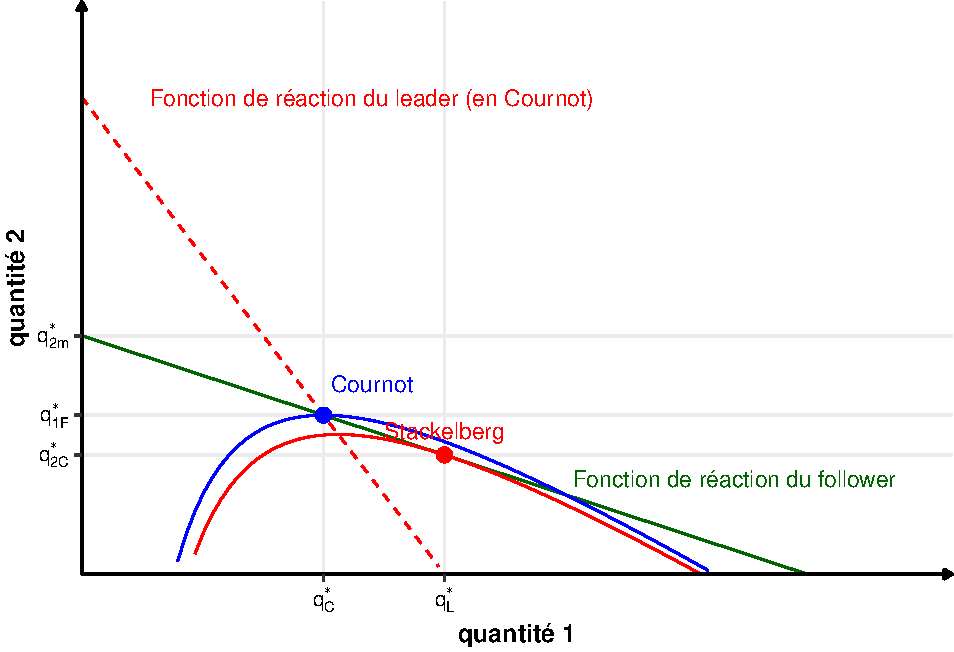
\includegraphics{_main_files/figure-latex/equilibreStackelberg-1.pdf}
\caption{\label{fig:equilibreStackelberg}Courbes d'isoprofits et fonctions de réactions des entreprises en équilibre de Stackelberg.}
\end{figure}

Sur la figure \ref{fig:equilibreStackelberg}, on voit que le profit du leader est plus important en Stackelberg qu'en Cournot (et l'inverse pour le follower).
Les quantités produites par l'entreprise leader sont plus importantes en Stackelberg qu'en Cournot, mais celle du follower sont plus faible.
La somme des deux est plus importante (\(q_{1C}^*+q_{2C}^*<q_{L}^*+q_{F}^*\)).
Le prix sera donc plus faible pour les consommateurs.

\hypertarget{exemple-1}{%
\subsection{Exemple}\label{exemple-1}}

\hypertarget{donnuxe9es-du-probluxe8mes}{%
\subsubsection{Données du problèmes}\label{donnuxe9es-du-probluxe8mes}}

Notons les variables et fonctions du leader avec un indice \(L\) et celles du follower avec un indice \(F\).

Gardons une fonction de demande linéaire.

\[
P(q_L+q_F) = a - b(q_L+q_F)
\]

Supposons, afin de simplifier les calculs, que les coûts marginaux sont nuls.

\hypertarget{profits-1}{%
\subsubsection{Profits}\label{profits-1}}

On en déduit les profits :

\[
\begin{array}{rcl}
\pi_L(q_L, q_F) &=& \left(a-b(q_L+q_F)\right)q_L\\
\pi_F(q_L, q_F) &=& \left(a-b(q_L+q_F)\right)q_F
\end{array}
\]

\hypertarget{fonction-de-ruxe9action-de-lentreprise-follower}{%
\subsubsection{Fonction de réaction de l'entreprise follower}\label{fonction-de-ruxe9action-de-lentreprise-follower}}

Calculons la fonction de réaction de l'entreprise follower.
La condition du premier ordre suivant \(q_F\) s'écrit (ici \(q_L\) est considéré comme une donnée par l'entreprise 1) :

\[
\begin{array}{crcl}
&\frac{\partial \pi_F}{\partial q_F}&=&0\\
\Leftrightarrow & (a-bq_L)-2bq_F^* &=& 0\\
\Leftrightarrow & q_F^* &=& \frac{a-bq_L}{2b}
\label{eq:FRFollower}
\end{array}
\]

\hypertarget{maximisation-de-lentreprise-leader}{%
\subsubsection{Maximisation de l'entreprise leader}\label{maximisation-de-lentreprise-leader}}

Comme l'entreprise leader connaît la fonction de réaction de l'entreprise follower (donnée par l'équation \eqref{eq:FRFollower}), elle peut l'intégrer à sa propre fonction de profit :

\[
\begin{array}{rcl}
\pi_L(q_L, q_F^*) &=& \left(a-b(q_L+q_F^*(q_L))\right)q_L\\
 &=& \left(a-b\left(q_L+\frac{a-bq_L}{2b}\right)\right)q_L\\
 &=& \frac{a}{2}q_L-\frac{b}{2}q_L^2
\end{array}
\]

La condition de premier ordre du leader est :

\[
\begin{array}{crcl}
&\frac{\partial \pi_L}{\partial q_L}&=&0\\
\Leftrightarrow & \frac{a}{2}-bq_L^* &=& 0\\
\Leftrightarrow & q_L^* &=& \frac{a}{2b}
\end{array}
\]

On en déduit qu'à l'équilibre de Stackelberg, le follower produit :
\[
q_F^*=\frac{a}{4b}
\]

L'entreprise leader produit plus que l'entreprise follower.
Elle profite de son pouvoir sur la seconde entreprise pour cela.
Si on calcule le profit, on verra que le profit de l'entreprise leader est plus important que celui de l'entreprise follower si elles sont exactement symétriques, en dehors de leur prises de décisions.

\hypertarget{cartels-et-collusions}{%
\section{Cartels et collusions}\label{cartels-et-collusions}}

\hypertarget{introduction-3}{%
\subsection{Introduction}\label{introduction-3}}

En duopoles / oligopoles de Cournot ou de Stackelberg, les entreprises ne coopèrent pas entre elles :

\begin{itemize}
\tightlist
\item
  Elles sont en concurrence ;
\item
  Elles agissent indépendamment les unes des autres.
\end{itemize}

\emph{Question :}\\
Que se passe-t-il si elles peuvent s'entendre ?
Par exemple, que se passe-t-il si elle peuvent passer un accord sur la quantité à produire.

\emph{Résultats :}\\
Les quantités mises sur le marché vont diminuer, et le prix du marché va augmenter.
C'est donc néfaste pour les consommateurs.
La raison est que le cartel se comporte exactement comme un monopole, puis partage les bénéfices.

\hypertarget{raisonnement-graphique}{%
\subsection{Raisonnement graphique}\label{raisonnement-graphique}}

\hypertarget{ruxe9solution-analytique}{%
\subsection{Résolution analytique}\label{ruxe9solution-analytique}}

\hypertarget{iduxe9e}{%
\subsubsection{Idée}\label{iduxe9e}}

L'idée derrière la résolution analytique du problème du cartel est de considérer que le cartel se comporte comme un monopole avec 2 centres de productions.
Le cartel choisit la quantité globale produite et la répartition entre les entreprises.
C'est un raisonnement très similaire à un monopole discriminant au troisième degré.

\hypertarget{profits-2}{%
\subsubsection{Profits}\label{profits-2}}

Le profit global du cartel s'écrit :
\[
\pi_c=qP(q)-C_A(q_A)-C_B(q_B)=(q_A+q_B)P(q_A+q_B)-C_A(q_A)-C_B(q_B)
\]
Où \(q=q_A+q_B\).
Le profit est maximisé lorsque les dérivées partielles suivant chacune des quantités sont nulles (condition du premier ordre), c'est-à-dire lorsque \(\frac{\partial\pi_C}{\partial q_A}=0\) et \(\frac{\partial\pi_C}{\partial q_B}=0\).
\[
\frac{\partial\pi_C}{\partial q_A} = P(q) + q\frac{\partial P}{\partial q}(q_A)-\frac{\partial C_A}{\partial q_A}(q_A)
\]
On a \(P(q) + q\frac{\partial P}{\partial q}=R_m(q)\) est la recette marginale totale du cartel.
\(\frac{\partial C_A}{\partial q_A}=C_{mA}\) est le coût marginal de l'entreprise A.\\
On peut réécrire la dérivée du profit total suivant la quantité produite par l'entreprise A :
\[
\frac{\partial\pi_C}{\partial q_A} = R_m(q)  - C_{mA}(q_A)
\]
En utilisant le même raisonnement, on a pour l'entreprise B :
\[
\frac{\partial\pi_C}{\partial q_B} = R_m(q)  - C_{mB}(q_B)
\]

\hypertarget{optimalituxe9-pour-le-cartel}{%
\subsubsection{Optimalité pour le cartel}\label{optimalituxe9-pour-le-cartel}}

A l'optimum pour le cartel, on a donc :
\[R_m(q) = C_{mA}(q_A) = C_{mB}(q_B)\]
Le cartel égalise la recette marginale \emph{totale} aux coûts marginaux de chacune des deux entreprises.

\emph{Remarque :} Le cartel ne va pas forcément donner à produire la même quantité à chaque entreprise.
La répartition dépend des coûts marginaux respectifs.
Si les coûts marginaux sont identiques, les productions seront identiques.

\emph{Intuition :} Supposons que la quantité totale produite est fixée.
Supposons aussi que \(C_{mA}(q_A)>C_{mB}(q_B)\).\\
Alors, en transférant la production d'une unité de l'entreprise A vers l'entreprise B, le coût diminue de \(C_{mA}(q_A)\) et augmente de \(C_{mB}(q_B)\).
Il diminue donc au total, tout en maintenant la même quantité totale produite.\\
Autrement dit, tant que \(C_{mA}(q_A)\neq C_{mB}(q_B)\), il est possible de diminuer le coût total de production d'une quantité donnée en répartissant celle-ci différemment entre les entreprises.

\hypertarget{optimalituxe9-pour-une-entreprise}{%
\subsubsection{Optimalité pour une entreprise}\label{optimalituxe9-pour-une-entreprise}}

\emph{Question :} Prenons l'entreprise A, a-t-elle intérêt à rester dans le cartel (et à respecter la répartition donnée par celui-ci) ?

Le profit de l'entreprise A s'écrit :
\[
\pi_A=q_AP(q)-C_A(q_A)=q_AP(q_A+q_B)-C_A(q_A)
\]
La dérivée du profit s'écrit donc :
\[
\frac{\partial\pi_A}{\partial q_A}(q_A)=P(q_A+q_B)+q_A\frac{\partial P}{\partial q}(q_A)-C_{mA}(q_A)
\]
La condition d'optimalité du cartel suivant \(q_A\) donne :
\[
\begin{array}{crcl}
& P(q_A^*+q_B^*) + (q_A^*+q_B^*)\frac{\partial P}{\partial q}(q_A^*)-\frac{\partial C_A}{\partial q_A}(q_A^*)& = &0\\
\Leftrightarrow &  P(q_A^*+q_B^*) + q_A^*\frac{\partial P}{\partial q}(q_A^*)-\frac{\partial C_A}{\partial q_A}(q_A^*)& = &-q_B^*\frac{\partial P}{\partial q}(q_A^*)\\
\Leftrightarrow & \frac{\partial\pi_A}{\partial q_A}(q_A^*)& =  &-q_B^*\frac{\partial P}{\partial q}(q_A^*)
 \end{array}
\]
Or on sait que la fonction de demande inverse \(P(q)\) est décroissante avec les quantités produites, ou que la fonction de demande est décroissante avec le prix, ce qui revient au même.
Donc \(\frac{\partial P}{\partial q}(q_A)<0\).
On en déduit donc que \(\frac{\partial\pi_A}{\partial q_A}(q_A^*)>0\) : l'entreprise A a intérêt à augmenter sa production si elle pense que l'entreprise B va respecter l'accord du cartel (et réciproquement).

En conclusion, les accords de cartel ne sont pas ``naturellement'' stable, ils ont besoin d'un mécanisme qui maintient l'accord, par exemple en punissant une entreprise déviant de l'accord.

  \bibliography{book.bib,packages.bib,bibliographie.bib}

\end{document}
